% Created 2015-08-09 su 18:45
\documentclass[12pt,a4paper,english]{tutthesis}
% Note that you must choose either Finnish or English here and there in this
% file.
% Other options for document class
  % ,twoside,openright   % If printing on both sides (>80 pages)
  % ,twocolumn           % Can be used in lab reports, not in theses

% Ensure the correct Pdf size (not needed in all environments)
\special{papersize=210mm,297mm}


% LaTeX file for BSC/MSc theses and lab reports.
% Requires the class file (=template) tutthesis.cls, tut-logo,
% exampleFig (as pdf or eps) and example_code.c
% Author: Sami Paavilainen (2006)
% Modified: Heikki Huttunen (@tut.fi) 2012-07-31
%           Erno Salminen   (@tut.fi) 2014-08-15
%             - added text snippets from the writing guide
%             - added lots of comments: both tips and alternative styles
%             - added an example table
%             - and so on...

%
% Define your basic information
%
\author{Riku Itäpuro}
\title{Thesis title}      % primary title (for front page)
\titleB{Otsikko suomeksi} % translated title for abstract
\thesistype{Master of Science thesis} % or Bachelor of Science, Laboratory Report... 
\examiner{Vilma Valkky} % without title Prof., Dr., MSc or such

% Special trick to use internal macros outside the cls file
% (e.g. @author). Trick is reversed with makeatother a bit later.
\makeatletter

% Define the pdf document properties
\hypersetup{   
  pdftitle={\@title},
  pdfauthor={\@author},
  pdfkeywords={transmogrifier design analysis}
}
\usepackage[finnish, english]{babel}


\author{Riku Itäpuro}
\title{Smartphone as a trust anchor for delegated home net configuration management}
\titleB{Älypuhelin kotiverkkojen luottamusankkurina}
% Ensure the correct Pdf size (not needed in all #+LATEX_HEADER: \special{papersize=210mm,297mm}
\thesistype{draft-7.8.2015 Master of Science thesis}
\examiner{Jarmo Harju}
\makeatletter
\usepackage[utf8]{inputenc}
\usepackage[all]{nowidow}
\author{Riku Itäpuro}
\date{7.8.2015  \{27.7,11.5,7.5.to the github,28.4, 16.4, 13.4.2015 new-framing, 4.4, 27.3,  20.3, 7.3)}
\title{Smartphone as a trust anchor in home networks}
\hypersetup{
  pdfkeywords={},
  pdfsubject={},
  pdfcreator={Emacs 24.4.1 (Org mode 8.2.10)}}
\begin{document}

\maketitle



 \hypersetup{  
 pdfkeywords={authentication, authorization, AAA, homenet, smartphone, trust anchor, EAP-SIM, RADIUS}
}
\chapter*{Terminology}
%\chapter*{Lyhenteet ja merkinn<E4>t}
\markboth{}{}                                % no headers

If not already on vocabulary, expansion of the most important terms like
authentication, key-exchange, integrity, replay, algorithms, SIM,\ldots{}
[from Cryptoprotocol-course, check that key exchange with 8 different methods)]

\newpage             % Added 2015-02-22

 \pagenumbering{Roman}
 \pagestyle{headings}
% \begin{document}
%  title page 
 \thispagestyle{empty}
\date\today
 \vspace*{-.5cm}\noindent
 
\includegraphics[width=8cm]{tty_tut_logo}   % Bilingual logo

% lay out author, title and type 
\vspace{6.8cm}
\maketitle
%\vspace{7.7cm} % -> 6.7cm if thesis title needs two lines
\vspace{6.7cm} % -> 6.7cm if thesis title needs two lines

% Last some additional info to the bottom-right corner
\begin{flushright}  
  \begin{minipage}[c]{6.8cm}
    \begin{spacing}{1.0}
      %\textsf{Tarkastaja: Prof. \@examiner}\\
      %\textsf{Tarkastaja ja aihe hyväksytty}\\ 
      %\textsf{xxxxxxx tiedekuntaneuvoston}\\
      %\textsf{kokouksessa 4.2.2015}\\
      \textsf{Examiner: Prof. \@examiner}\\
      \textsf{Examiner and topic approved by the}\\ 
      \textsf{Faculty Council of the Faculty of} \\
      \textsf{Computing and Electrical Engineering} \\
      \textsf{on 4th February 2015}\\
    \end{spacing}
  \end{minipage}
\end{flushright}


% Leave the backside of title page empty in twoside mode
\if@twoside
\clearpage
\fi


\pagenumbering{roman}
\setcounter{page}{0} % Start numbering from zero because command 'chapter*' does page break

%%% \begin{otherlanguage}{english} %  Following text in in 2nd language
\chapter*{Abstract}

\begin{spacing}{1.0}
  {\bf \textsf{\MakeUppercase{\@author}}}: \@title\\   % use \@titleB when thesis is in Finnish
   \textsf{Tampere University of Technology}\\
   \textsf{\@thesistype, xx pages, x Appendix pages} \\
   \textsf{xxxxxx 2015}\\
   \textsf{Master's Degree Programme in Information Technology}\\
   \textsf{Major: Information Security}\\
   \textsf{Examiner: Prof. \@examiner}\\ % 
   \textsf{Keywords: authentication, authorization, AAA, homenet, smartphone, SIM, trust-anchor, EAP-SIM, RADIUS}\\
\end{spacing}

%---------------------------------------------------------
%   A B S T R A C T
% [The abstract is a concise 1-page description of the work: 
[what was the problem, what was done, and what are the results. ]
% Do not include charts or tables in the abstract.


Home network devices can be configured by different means but usually one needs 
to have some knowledge how to login to those devices. For that, 
some beforehand set provisioning and distribution of authentication keys is needed.

As there already exists an infrastructure within mobile phone subscribers,
that is used in the study as a trusted base.
% To benefit from mobile identification
To benefit from mobile identification it is shown how
%It is discussed and shown how mobile authentication 
%it is done using extendable authentication profile (EAP) with SIM-card. 
 authentication  is done using extendable authentication profile (EAP) with SIM-card
and authorization checked with RADIUS protocol.




A theory, how SIM-authentication works is presented and a simulated environment
to demonstrate that is built, tested and analyzed.
As a result it is shown, that SIM authentication's benefits are strong
authentication and existing user-base, while its disadvantages include
dependency to mobile operator. Additionally, there will remain challenges in keeping SIM's identity private and in disabling unwanted re-authentications. 
% [or: balancing the re-authentication]

Principle has been to reuse existing techniques when combining them to such new areas as homenet and delegated management.
 For transporting authentication claims, WPA2 enterprise has been chosen, which includes RADIUS environment.
To further avoid complexity and granularity, we
only use a simple model of management network. Getting in to management network is carried out at homenet via EAP-SIM authentication and it is the key element of the thesis.



%%%\end{otherlanguage} % End on 2nd language part
%---------------------------------------------------------
%   T I I V I S T E L M Ä 

\begin{otherlanguage}{finnish} %  Following text in in 2nd language
\chapter*{Tiivistelmä}         % Asterisk * turns numbering off

\begin{spacing}{1.0}
         {\bf \textsf{\MakeUppercase{\@author}}}: \@titleB\\  % or use \@title when thesis is in Finnish
         \textsf{Tampereen teknillinen yliopisto}\\
         \textsf{Diplomityö, xx sivua, x liitesivua}\\ %
         \textsf{toukokuu 2015}\\
         \textsf{Tietotekniikan koulutusohjelma}\\
         \textsf{Pääaine: tietoturva}\\
         \textsf{Tarkastaja:  Prof. \@examiner}\\ % automated, if just 1 examiner
         \textsf{Avainsanat: tunnistaminen, valtuutus, AAA, kotiverkko, älypuhelin, luottamusankkuri, EAP-SIM, RADIUS}\\
\end{spacing}
The abstract in Finnish. Foreign students do not need this page.
TBD

Kirjoita, kun english versio on hyvä(ksytty).
\end{otherlanguage} % End on 2nd language part

% varmuuden vuoksi, sillä esim. captioneissa Kuva tulee muuten suomeksi 
%%% \begin{otherlanguage}{english} %  Following text in in 2nd language
\begin{otherlanguage}{english} %  Following text in in 2nd language
\makeatother % Make the @ a special symbol again, as \@author and \@title are not neded after this

%
% PREFACE
%
\chapter*{Preface}

PREFACE TEMPLATE! SKIP.

This document template conforms to Guide to Writing a Thesis at
Tampere University of Technology (2014) and is based on the previous
template. The main purpose is to show how the theses are formatted
using LaTeX (or \LaTeX ~ to be extra fancy) .


The thesis text is written into file \texttt{d\_tyo.tex}, whereas
\texttt{tutthesis.cls} contains the formatting instructions. Both
files include lots of comments (start with \%) that should help in
using LaTeX. TUT specific formatting is done by additional settings on
top of the original \texttt{report.cls} class file. This example needs
few additional files: TUT logo, example figure, example code, as well
as example bibliography and its formatting (\texttt{.bst}) An example
makefile is provided for those preferring command line. You are
encouraged to comment your work and to keep the length of lines
moderate, e.g. <80 characters. In Emacs, you can use \texttt{Alt-Q} to
break long lines in a paragraph and \texttt{Tab} to indent commands
(e.g. inside figure and table environments). Moreover, tex files are
well suited for versioning systems, such as Subversion or Git.  
% \url{http://www.ctan.org/tex-archive/info/lshort/english/lshort.pdf}

Acknowledgements to those who contributed to the thesis are generally
presented in the preface. It is not appropriate to criticize anyone in
the preface, even though the preface will not affect your grade. The
preface must fit on one page. Add the date, after which you have not
made any revisions to the text, at the end of the preface.

~ 
% Tilde ~ makes an non-breakable spce in LaTeX. Here it is used to get
% two consecutive paragraph breaks

Tampere, 1.5.2015
~


Teemu Teekkari
%
% Add the table of contents, optionally also the lists of figures,
% tables and codes.
%

\renewcommand\contentsname{Table of Contents} % Set English name (otherwise bilingual babel might break this), 2014-09-01
%\renewcommand\contentsname{Sis<E4>llys}         % Set Finnish name
\setcounter{tocdepth}{3}                      % How many header level are included

%% ei tähän vielä 
% latexin \tableofcontens clearaa yhden käytön jälkeen, siksi tässä tyhjä.
% Yritä kieltää se ennen tätä.
% ks. http://orgmode.org/manual/Table-of-contents.html
\tableofcontents                              % Create TOC

\renewcommand\listfigurename{List of Figures}  % Set English name (otherwise bilingual babel might break this)
%\renewcommand\listfigurename{Kuvaluettelo}    % Set Finnish name
\listoffigures                                 % Optional: create the list of figures
\markboth{}{}                                  % no headers

\renewcommand\listtablename{List of Tables}    % Set English name (otherwise bilingual babel might break this)
%\renewcommand\listtablename{Taulukkoluettelo} % Set Finnish name
\listoftables                                  % Optional: create the list of tables
\markboth{}{}                                  % no headers


%\renewcommand\lstlistlistingname{List of Programs}      % Set English name (otherwise bilingual babel might break this)
%%\renewcommand\lstlistlistingname{Ohjelmaluettelo} % SetFinnish name, remove this if using English
\lstlistoflistings                                % Optional: create the list of program codes
%\markboth{}{}                                     % no headers


%
% Term and symbol exaplanations use a special list type
%

\chapter*{List of abbreviations and symbols}
%\chapter*{Lyhenteet ja merkinn<E4>t}
\markboth{}{}                                % no headers

% You do not have to align these with whitespaces, but it makes the
% .tex file more readable
\begin{termlist}
% \item [CC license] Creative Commons license
% \item [LaTeX]      Typesetting system for scientific documentation
% \item [SI system]  Syst\`eme international d'unit's, International System of Units
\item [TUT]    Tampere University of Technology
\item [URL]    Uniform Resource Locator
\item[3GPP] $3^{rd}$ Generation Partnership Project
\item[AAA] Authentication, Authorization, Accounting
\item[AKA] Authentication and Key Agreement %, used in 3GPP mobile networks 
\item[AUC] AUthentication Center
\item[CPE] Customer Premise Equipment %, device physically located at customers home.
\item[EAP] Extensible Authentication Protocol %, extends 802.1X
\item[GAA] Generic Authentication Architecture % (for SSO)
\item[GBA] Generic Bootstrapping Architecture
\item[GSM] Global System for Mobile Communication (earlier Groupe Spécial Mobile)
\item[HLR] Home Location Registry, ...
% \item[ICCID] card serial
\item[IEEE] Institute of Electrical and Electronics Engineers
\item[IMSI] International Mobile Subscriber Identity
\item[ISP] internet service provider
\item[MNO] mobile network operator, owner of cellular network, knows SIM secrets
\item[RADIUS] Remote Authentication Dial In User Service, protocol and server,  AAA service 
\item[SIM]  Subscriber Identity Module, a smartcard. Also USIM program running in UICC card (UMTS networks)
\item[SSID] Service Set Identifier, identifies Wi-Fi network
\item[TMSI] Temporal Mobile Subscriber Identity
\item[Wi-Fi] Wireless local network, implements IEEE 802.11 standards
\item[WPA] Wireless Protected Access version 1.
\item[WPA2] Wireless Protected Access version 2, more secure than WPA
\end{termlist} 


% The abbreviations and symbols used in the thesis are collected into a
% list in alphabetical order. In addition, they are explained upon
% first usage in the text.

\begin{description}
\item[{802.1X}] port based access control standard
\item[{Access point}] Wi-Fi client connects access point (AP) on 802.11
layer. AP knows EAP client and encapsulates EAP-message
to RADIUS-message and forwards that to
Authenticator.
\end{description}
\begin{description}
\item[{Authenticator}] local entity, who makes authentication (and
authorization) decision for client based on local and remote
claims, part of 802.1X standard.
\end{description}
\begin{description}
\item[{mobile-operator}] knows connection between SIM-owner and SIM
\end{description}
\begin{description}
\item[{proxying RADIUS}] RADIUS server standing between RADIUS
client and Authentication server, part of RADIUS server chain.
\end{description}



% The actual text begins here and page numbering changes to 1,2...
% Leave the backside of title empty in twoside mode
\if@twoside
\cleardoublepage
\fi

\newpage             % Added 2014-09-01
\pagenumbering{arabic}
\setcounter{page}{1} % Start numbering from zero because command
                     % 'chapter*' does page break
\renewcommand{\chaptername}{} % This disables the prefix 'Chapter' or
                              % 'Luku' in page headers (in 'twoside'
                              % mode)

\chapter{Introduction}
\label{sec-1}
\label{cha:intro}


Managing computer and network devices can be hard.  Modern homes have
become similar to small offices regarding the equipment present there.
Earlier it was sufficient to make just minimal settings at home to a
modem (cable, phone or radio) and connect it to the home computer to
get a fully working home network with internet connectivity.  Now home
network has expanded with countless devices available.  Already
entertainment centers (AV-amplifiers, media players, gameconsoles),
manageable network devices (switches/routers), and mobile phones
present new devices and network segments beside computers and
printers. Sensors and controller devices from Internet of Things
domain bring their own increment to the device count at home.

Connecting these devices to the net remains trivial, but managing the
network afterwards has become challenging and complex.

There might be separate areas in homes that have different needs regarding
connectivity, resources, and access. Not only that, but devices in
separate segments might not belong to the home owner anymore, hence needing
their own administrative parties. For example an electricity company may
have a sensor and controller network, which physically uses the home network, but
logical is separated from other parts of home network. It is then
important to keep track of who is allowed to access which part of the
home network. 


The configuration choices in networking devices takes some
amount of expertise what is not necessarily present at every
home. There could exist a market for an external consultant service, which would
remotely operate the home network.
Remote operation eliminates consultant's 
physical precence at home and so reduces external actors' costs, but adds many questions
regarding security, not only to overcome firewalls, NATs, and disconnections.
Persons, who are allowed to make configuration changes, are today
often authenticated only by simple password and physical precence at home.
If external help were present, home owner would need more 
control allowing only authorized operators in, because earlier used
physical precence protection is missing.

Lastly, it is challenging to find a common, 
trusted entity, upon which every actor could base their trust.
Common trust is needed to join before unknown parties together
safely. 

Summarized the problems are a delegated network management, remote
provisioning, and trust finding. On its roots, it is an authentication
and authorization problem.










One model to solve these problems is to separate the management and
control function away from the connectivity and routing
issues. Silverajan et al.\cite{silverajan2015collaborative} proposes
model where management is achieved through a service in a cloud. The
configuration model of devices at a home is mirrored to the cloud as a
resource graph ( Figure x.1) and changes can be planned ahead at cloud
and committed (Pushed) later to the home via a local controller point
which lies at home using configuration tools CoAP and RESTCONF.
(Figure x.2).

The cloud have already verified the operators in the cloud, but the
question remains, how to connect the cloud service to the home network
through the local controller securely. The local controller at home
would approve the changes and a smartphone is assumed to function in
local controller role. It will have an application which operates as a
bridge and an access control between the cloud and the home network.
See Figure\ref{fig:localcontroller} for design of this architecture.

\begin{figure}[htb]
\centering
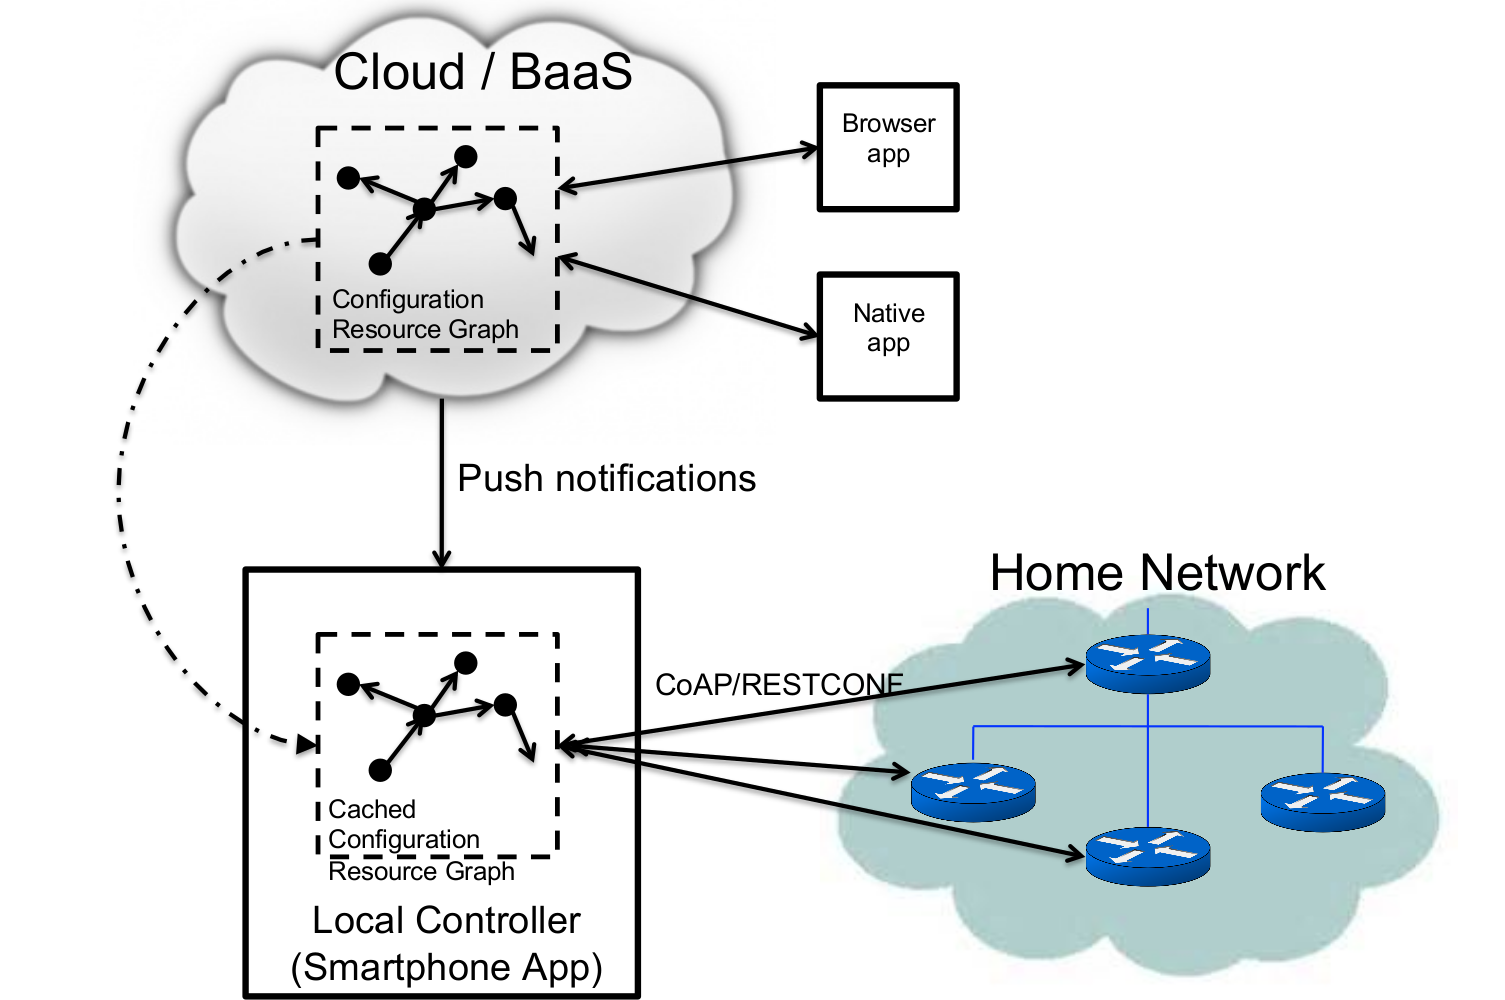
\includegraphics[width=.9\linewidth]{/home/itapuro/gitdocs/di/images/localcontroller.png}
\caption{\label{fig:localcontroller}Local Controller and Collaborative Management Design}
\end{figure}


The delegated service provider therefore does not need to have a direct data
access to the home but only to the cloud based service in order to be able to
manage homenet devices.
Consultant service is not the only possible delegation for home network.








One of the security issues is the authentication and authorization 
from the cloud to the home net.
To secure the connection from the cloud service (controller)
to the homenet, there needs to be a common trust between each end
point and the research problem here is how to enable the trust between the
controller and the homenet as the controller lies at the edge of the
home network.


Any encryption between devices needs trusted key exchange beforehand,
and finding and establishing trust is needed for that.  That is called
the key distribution problem. Public keys solve key exchange part, but
only partially, because the trust must still be found somewhere.
Above mentioned cloud solution at TUT for delegated home network
management currently has preliminary authentication and access model
using pre-defined credentials and SSH-connection from the local
controller device to configuration
targets\cite[Chap.4]{silverajan2015collaborative}.
That work does not yet handle the bootstrap of the infrastructure
i.e. the first trust is thought as given.  Smartphone with its SIM
card and existing key infrastructure to mobile network operator would
later eliminate the requirement for an additional credential
distribution and that issue is studied in this thesis.
Although mobile phone provides alternative
authentication method with its SIM key, usual methods to
authenticate still are plain username-password combinations.
Those security issues must be solved before delegation in the cloud can
happen.  








One motivator to this work is to find why SIM-based methods are not in
wider use.  The technology has been there for more than ten years and
the hardware and the applications mostly support it, but it still is
not yet widely used.  Could there exist a light method to use the SIM?




The trust can be derived from facts that already are known.  The
place, where a trust is not anymore derived or built upon other fact
but assumed to be present, is called a trust anchor.  
[OR: \emph{The trust anchor is then the fact, state or place,
where derivation is done no more, but accepted per se.} ]
Combining existing techniques, this thesis presents one possible way
to bind home network's trust to the smartphone's unique, existing
secret keys inside the smart card's Subscriber Identify Module (SIM),
which then would function as a trust anchor. To generally find
ultimate trust it is only needed to verify trust chains until the
chain reaches a trust anchor.


Human aspect and usability are important, although the focus will
still be on authentication and authorization part of the home net
management with smartphone as trust anchor.  The proposed model
should nevertheless require less effort than the current used methods
on distributing user credentials, finding right place for them to be
inserted, and ensuring that they are written correctly.
Besides those, problems such as limited connectivity are
studied.





The thesis is structured as follows: Chapter \ref{sec-2} explains the
authentication-authorization model.  Chapter \ref{sec-3} describes
security in current home net architecture and current practices for
configuring it.  Chapter \ref{sec-4} discusses methods to bring a
trust anchor in the homenet and explains the chosen method.
One specially crafted problem is how the scenarios presented here can be
tested without knowing SIM card's secret keys and without real phone
operator involved.  Those experiments are described in Chapter
\ref{sec-5}.
Results are discussed on Chapter \ref{sec-6} and Chapter \ref{sec-7} concludes the
thesis.
\chapter{Authentication, Authorization, and Trust}
\label{sec-2}

[TBD 4) Feature comparison, eg role-based access, time-based access
etc]

[TBD 5) GBA and Security bootstrapping]

Authentication, authorization, and accounting services (AAA) are
components for access management.  AAA-protocols do not dictate
policies, i.e., who is granted access or what operations user is
allowed to do. They only transport this information between client
who needs them and server authorized to provide them.
Often, the last 'A' which stands for accounting has been neglected
and also here only first two A's are used and later described as AA
services. Authentication (AuthN) answers how to identify users and
prove that they really are who they claim to be. Authorization (AuthZ)
answers what operations the identified users are allowed to do and
forces usage policy. The rest of the thesis uses shortened terms AuthN
and AuthZ.

On very small environments AA service is built on static backend such
as file on protected target that the object wants to access. There AuthN
is checked against a credentials file and authorization from a service
specific policy file. 
To be more exact, identification preceding authentication is the part,
where entity claims and presents its identity to 
access controlling system. That can involve sending username, login
name or other identifier. Authentication in turn is the part where
those facts are verified. AuthZ involves checking, which rights are 
available for authenticated entity. 


Before we introduce SIM-based authentication used throughout the
thesis, protocols 802.1X, WPA2, EAP and RADIUS are described in the
following Sections.

\section{802.1X}
\label{sec-2-1}

802.1X\cite{8021X} is an IEEE standard protocol for port based access
control. Ports are physical layer ports, not to be mixed to Layer-4 ports such as TCP/UDP ports.
 Network access through a specific physical port is
restricted (controlled) from a client (called Supplicant) before
the client has successfully performed an AA. A 802.1X device, where
the ports are located, is called the Authenticator. Third party in 802.1X is an
Authentication server. 



It is easy to mix here terms \emph{Authenticator} and \emph{Authentication
server}, but their roles are different: Authenticator works as a
gate-keeper to ports between supplicant and network, while
Authentication server handles AA processes.
At home, Authenticator usually lies inside the access point, but 
on large enterprise networks, Authenticator can be a centralized unit 
and multiple access points function only as radio stations.



\section{RADIUS}
\label{sec-2-2}
\label{sec:radius}
RADIUS is the most popular provider for 
AAA-services\cite[p.75]{radius-popular}.  It was used first with remote terminal
and dial-up modem users, hence the name Remote Authentication Dial-In
User Service. Later it was used as centralized AAA for networking
devices such as switches and routers.  










RADIUS protocol is a stateless, request-response type client-server
protocol. 
There are four types of RADIUS messages defined in RFC 2865 that are
used in AA. ACCESS-REQUEST and ACCESS-CHALLENGE cover both AuthN and
AuthZ. As a result, the final RADIUS message will be either
ACCESS-ACCEPT or ACCESS-REJECT sent to the RADIUS client, based on the
result given by the RADIUS authentication server.

Today, RADIUS has some shortcomings and fixing them is not anymore
reasonable as developing has shifted to another AAA protocol called
Diameter, which is already in use in 3GPP and 4G
networks\cite{diameter}.  Nevertheless, as RADIUS is so wide-spread,
it is still used in lots of places instead of Diameter.  Currently,
the main environment of RADIUS, besides network managing, is wireless
connections (Wi-Fi) in enterprises and nationwide community
federations.


When local Wi-Fi groups in Finland such as ``SparkNet'', ``Langaton
Tampere'', or ``Wippies'' started to form in around 2005, they used
802.1X and RADIUS for AA. Those networks did still have as an
alternative AA method a captive portal technique, where user
first authenticates on WWW-page before getting an access.  802.1X and
RADIUS enabled users in those group to consult external,
central RADIUS server for authentication requests automatically,
without burden that captive portal brings.  The members of Wi-Fi
groups can use network anywhere, where the same uniform SSID (Service
Set IDentifier) was seen, i.e., roaming
became possible, if one found a familiar SSID outside home area.  Later, there were agreements between different local groups
to allow roaming and so federations were born.

As seen from federated Wi-Fi groups, RADIUS servers can be chained to
form a tree. The reasons for the chaining are load balancing and high
availability, centralization of locally distant servers, and
federation of different domains. In RADIUS trees, the messages are
chained and proxied to next RADIUS server, depending on the settings
on the proxying RADIUS server.


In the following chapters it is discussed how proxying servers take 
part in AA decisions. Of main interest there is, if it is possible 
to inject or modify AuthZ information in those proxying RADIUSes in
cases, where AuthN and AuthZ are provided from different
 places\cite{rfc2607}. Secondary goal is to universally divide AA regarding 
clients domain in the federation.




\section{WPA2}
\label{sec-2-3}

Wireless protected access (WPA or WPA2) protects traffic in wireless,
shared media, where everyone otherwise can simple listen all the radio traffic.
It enables both authenticated access and message
encryption between the smartphone and wireless access point (AP) by negotiating session keys
after 802.1X has opened the virtual port in AP for the smartphone.

WPA (version 1)  was an early subset of then upcoming 802.11i standard,
while WPA2 is the full implementation, also noted as IEEE
802.11i-2004, and the term WPA2 is used throughout the thesis.
Client software for 802.11i is called a WPA2-Supplicant and it is used
in wireless clients to communicate with the Authenticator. 

WPA2 has two modes of protection: one for groups with common, pre-shared
key (WPA2-PSK, also known as WPA2-Personal) and one for individuals
(WPA2-RADIUS, also known as  WPA2-Enterprise).  With WPA2-RADIUS, revoking
individual access is easier, but client setup slightly more
complicated than on WPA2-PSK, as seen on Table\ref{psk-enterprise}.

\begin{table}[htb]
\caption{\label{psk-enterprise}Comparison of WPA2-PSK and WPA2-ENTERPRISE modes}
\centering
\begin{tabular}{l|l|l}
Property & WPA2-PSK & WPA2-ENTERPRISE\\
\hline
for groups & x & \\
for individual &  & x\\
client setup & easy & intermediate\\
individual client revocation &  & x\\
\hline
\end{tabular}
\end{table}


\section{EAP}
\label{sec-2-4}

Instead of bringing new AuthN methods into 802.1X, it was 
extended with a modular framework called 
 EAP (Extensible Authentication Protocol)\cite{rfc5247}. 
Ramification of using EAP is considered good among researchers, as it
provides flexibility, indepence of underlying technology, whether
wireless or wired,  and integration with AAA infrastructures, although
it adds some amount of time for authentication.\cite{pereniguez10}.
Different authentication methods, for example hashed passwords, TLS
 certificates, or SIM/AKA using smartphone's SIM card,  can
be used with EAP.
This work uses EAP-SIM authentication method.


EAP describes only the messaging form, so EAP messages needs to
be encapsulated inside another protocol.  In Wi-Fi, between a smartphone
and an AP, EAP is encapsulated into 802.1X protocol (as EAPOL) or
into protected EAP(PEAP)\cite{peap} before sending
into air. In wired net EAP messages are encapsulated into RADIUS.

The encapsulation is described in Figure\ref{fig:eap-layers} where it
can be seen, that EAP messaging happens logically between the EAP peer
and the
Authentication server, but on a lower transport layer there is an EAP
Authenticator in between them, which transfers EAPOL messaging into
RADIUS message.





\begin{figure}[htb]
\centering
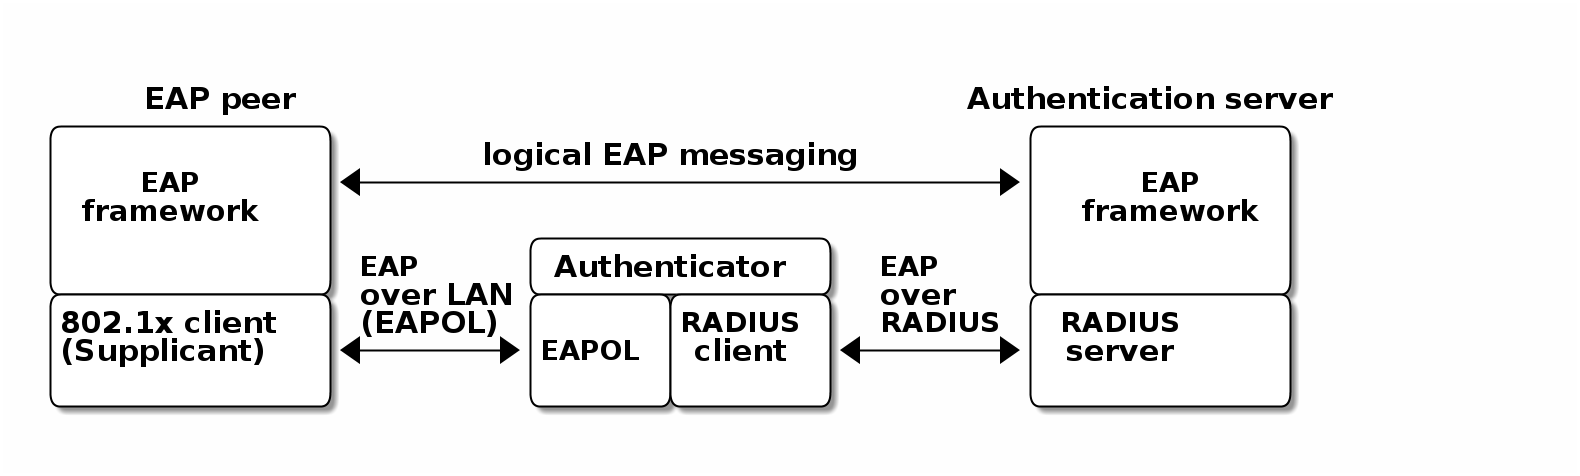
\includegraphics[width=.9\linewidth]{eap-layer.png}
\caption{\label{fig:eap-layers}EAP-logical layering}
\end{figure}


Further, EAP is used to transfer authentication messages only.
It does not include AuthZ information, which is RADIUS's
responsibility or session keys, which are negotiated by WPA2.  In the
end (not shown in the Figure\ref{fig:eap-layers}) of EAP messaging,
Authenticator is responsible for opening access for EAP peer as 802.1x
dictates.



\section{SIM-based authentication}
\label{sec-2-5}
\label{sec:sim-based-auth}
Usually, SIM is associated to a physical card used in smartphones to
bind a subscriber to the network operator.
SIM here means the secret keys and the application in mobile phone's
SIM or USIM inside UICC(Universal Integrated Circuit Card).
The secret keys are hardware protected and only usable to SIM card.
The SIM's storage also includes a unique serial number (ICCID) and a
unique IMSI (International Mobile Subscriber Identity).  SIM card usage
can be controlled by two passwords: PIN and PUK.  PUK is used as a
remedy, if PIN has been inserted wrong too many times.  If the card
has other applications, for example mobile electrical signature
application Mobiilivarmenne, they may have different keys and codes.


MNO distributes SIM card and provides mobile network connectivity to
its customer.  The secret keys are used for authenticating the IMSI
to MNO which enables MNO's to identify their customer in the network
and charge them correspondingly. It is assumed, that SIM card represent
its owner but in reality nothing prevents an identity thief to steal
someone's SIM card. Although 4-digit PIN tries to prevent the usage of 
stolen SIM, that is considered as a weak safe\cite[p.31]{aaa-nakhjiri2005}.


AA services need to trust some entity endpoint and in case of MNO and
SIM, they already mutually trust each other, and SIM can be used 
to open access to mobile networks.
There is still need for separate access credentials for Wi-Fi access
and that was the reason of developing EAP-SIM and later the
derivatives EAP-AKA and EAP-AKA'.  The goal was to combine in a secure
way existing keys used in  GSM (Global system for Mobile communication)
Wi-Fi access. Existing general purpose EAP-methods in 2004 were not
compatible with GSM protocols for this purpose. \cite[p.93]{hav-doc}
The result of development was that today SIM can be used via EAP-types EAP-SIM, EAP-AKA, or
EAP-AKA'(AKA-PRIME).

EAP-SIM is the original type created for GSM networks and defined 
in RFC4186\cite{rfc4186}.
It is a challenge-response method and similar to AuthN used in GSM, 
but adds mutual AuthN, i.e., also the network is authenticated.
Network authentication is achieved, if 
network is able to response correctly to a client sent nonce,
which by definition is a value used only once. The nonce can
be thought as  client's challenge to network.

The client in  turn is authenticated, when the Authentication server
generates a challenge with aid of triplet from MNO and the client
responses to it correctly.
That procedure is later described in more detail.

Beginning from 3GPP networks, new types EAP-AKA and AKA' can be used.
EAP-AKA is defined in RFC4187\cite{rfc4187} and 
 uses 3GPP's AKA (Authentication and Key Agreement) protocol.
It differs from EAP-SIM by using additionally parameters from MNO to
protect replay attacks. Otherwise the protocol messaging is same
as in  GSM-SIM, only algorithms differ.

Last, there exists EAP-AKA' that enhances AKA by including Service Set name (SSID) 
in the key derivation function, which limits the possibility of using possibly
compromised network's nodes and keys. Additionally, requests have
sequence numbering preventing replay attacks and its digests use SHA-256
function instead of SHA-1.\cite{rfc5448}.


  Using EAP-SIM means using the secret key inside SIM card with A3/A8
algorithms to generate valid responses for challenges coming from MNO
and to derive session keys.  The algorithms used (A3/A8) and their
possible implementations (COMP128, COMP128v2, COMPv3) are not of
interest in this work beside the point that they are MNO specific or known reference algorithms.


Disadvantages with SIM is dependency on mobile operator and internet
connection, although disconnectivity issues are later addressed partly.
Using smartphone may cost money, either to client or to service
provider, although costs could be lower than using SMS, because 
IP network is used instead of mobile phone network.

In many parts, SIM variants in EAP are simpler, than other EAP
variants to mobile client.  Table\ref{table-peapsim} compares the setup of Wi-Fi
in clients of one existing organization compared to EAP-SIM. It
is noteworthy, that plain EAP-SIM will not support identity hiding and
that will be later be discussed further. If we added PEAP
also to EAP-SIM (in last column of Table\ref{table-peapsim}), comparison would be more fair.
As can be seen from the table, leaving certificates out from the environment
makes client setup easier with the price of revealing smartphone user's
identity.  







\begin{table}[htb]
\caption{\label{table-peapsim}Setup tasks for clients in WPA2-Enterprise with EAP-PEAP-MSCHAPv2 and EAP-SIM}
\centering
\begin{tabular}{|l|l|l|ll|}
\hline
 & EAP-PEAP & EAP-SIM & EAP-PEAP & \\
Task: & with &  & with & \\
(x)=``needed'', (N/A)= ``not available'' & MSCHAPv2 &  & EAP-SIM & \\
\hline
CA settings: &  &  &  & \\
- choose CA for the RADIUS & x &  & x & \\
- tell CA to clients & x &  & x & \\
- if CA not known, distribute it \emph{securely} & x &  & x & \\
\hline
Other settings: &  &  &  & \\
- set used EAP-method & x & x & x & \\
- set validation of RADIUS server's name & x &  & x & \\
- set encapsulation (WPA2/802.1X) & x &  &  & \\
- set password & x & x(PIN) &  & \\
\hline
Identity hiding: &  &  &  & \\
- enable PEAP & x & N/A & x & \\
- set outer identity & x & N/A & x & \\
- set inner identity & x & N/A &  & \\
\hline
\end{tabular}
\end{table}





Unique identifier for SIM is IMSI (International Mobile Subscriber
Identity, 15 digits long, more familiar user's phone number.
Important parameters for this work are IMSI, NONCE, and triplet values
corresponding IMSI (RAND, SRES, Kc).

Sequence diagram of full EAP-SIM authentication between Supplicant (here
smartphone) and Authenticator (in AP) is shown in
Figure\ref{fig:eap-sim-full} . 
There we can see that IMSI is used in message 2. IMSI is the
identity, which Authentication server would next try to challenge and
for which the AuthZ would be checked.



All EAP-SIM derivatives provide mutual authentication.
An operator is authenticated, when the client challenges it by sending
a NONCE value during the start of the negotiation phase in the
message 4. The client later checks in the process 7., whether RAND
values from the operator were digested with the correct NONCE.

After session has been set, IMSI may be left out and instead a
temporal IMSI (TMSI) can be used to hide client's identity, for
example in re-authentication case. It must be noted, that this TMSI
differs from TMSI used in 3GPP network. Those context must not be
mixed, otherwise the security that they bring may reduce.
Unfortunately, IMSI has at that point already been exposed once in
plain text, namely in message 2.









\begin{figure}[htb]
\centering
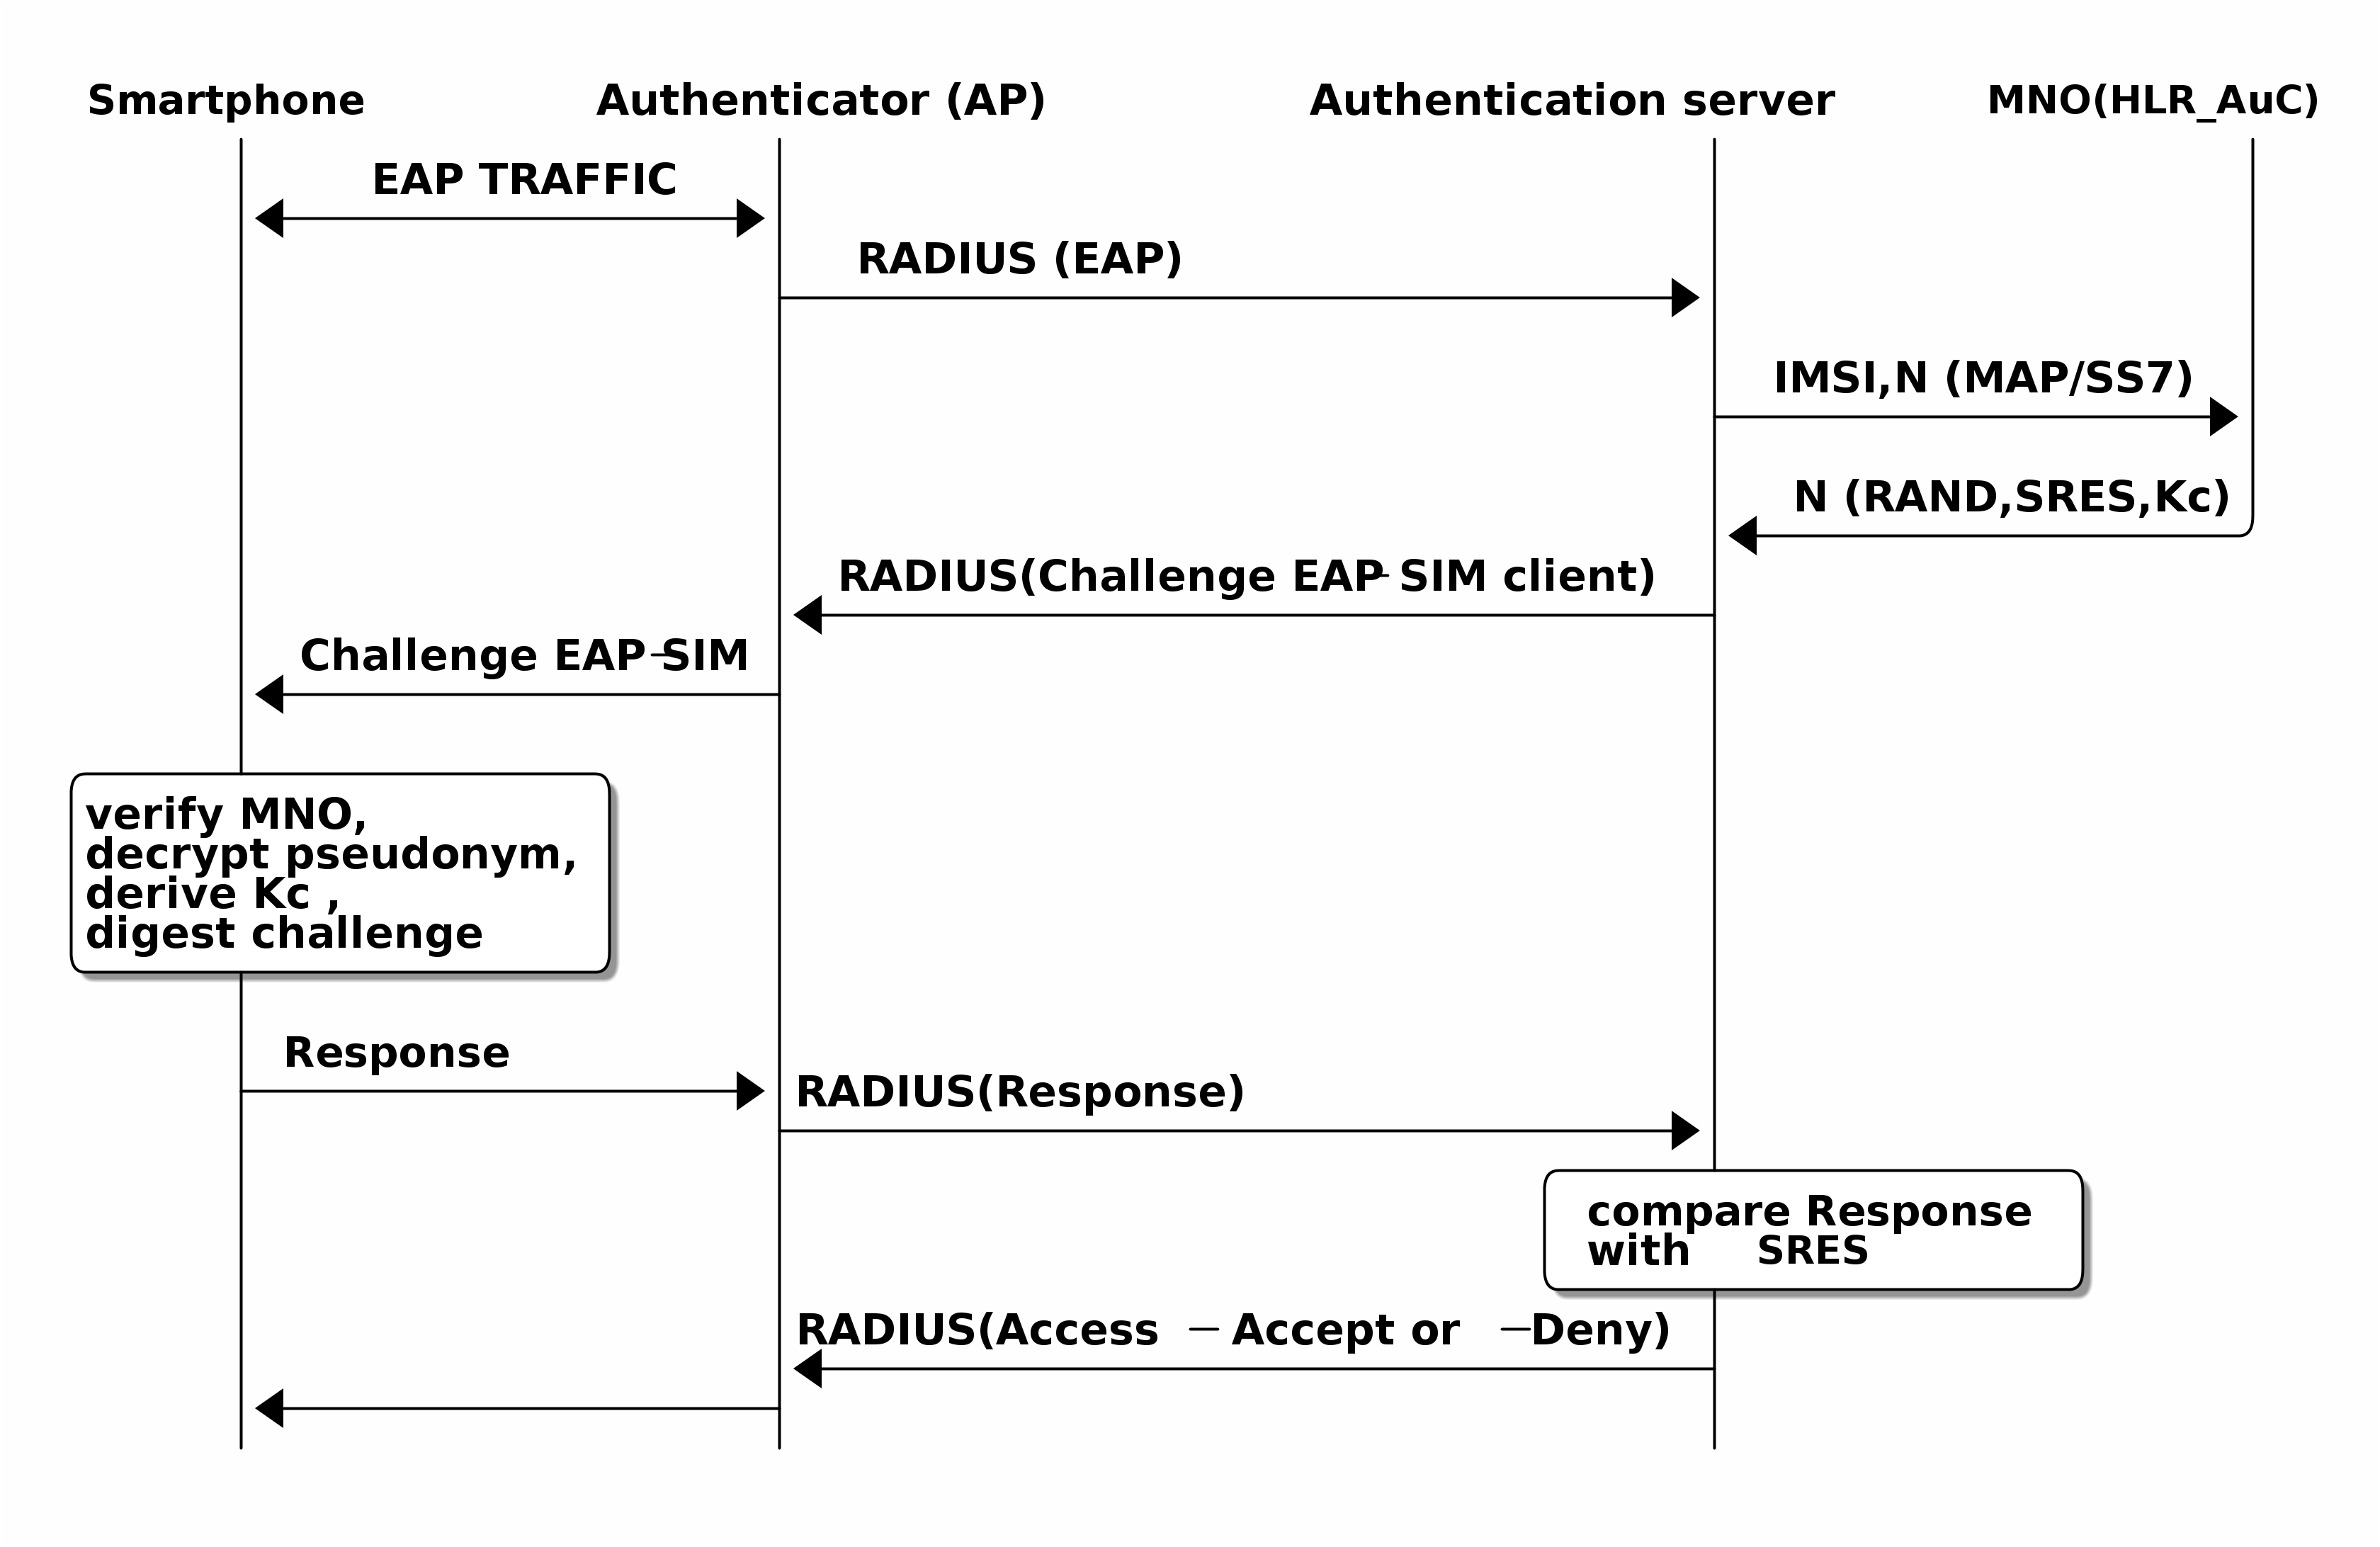
\includegraphics[width=.9\linewidth]{eap-sim-simple.png}
\caption{\label{fig:eap-sim-simple}Detailed EAP-SIM simplified sequence diagram, source RFC4186}
\end{figure}




\begin{figure}[htb]
\centering
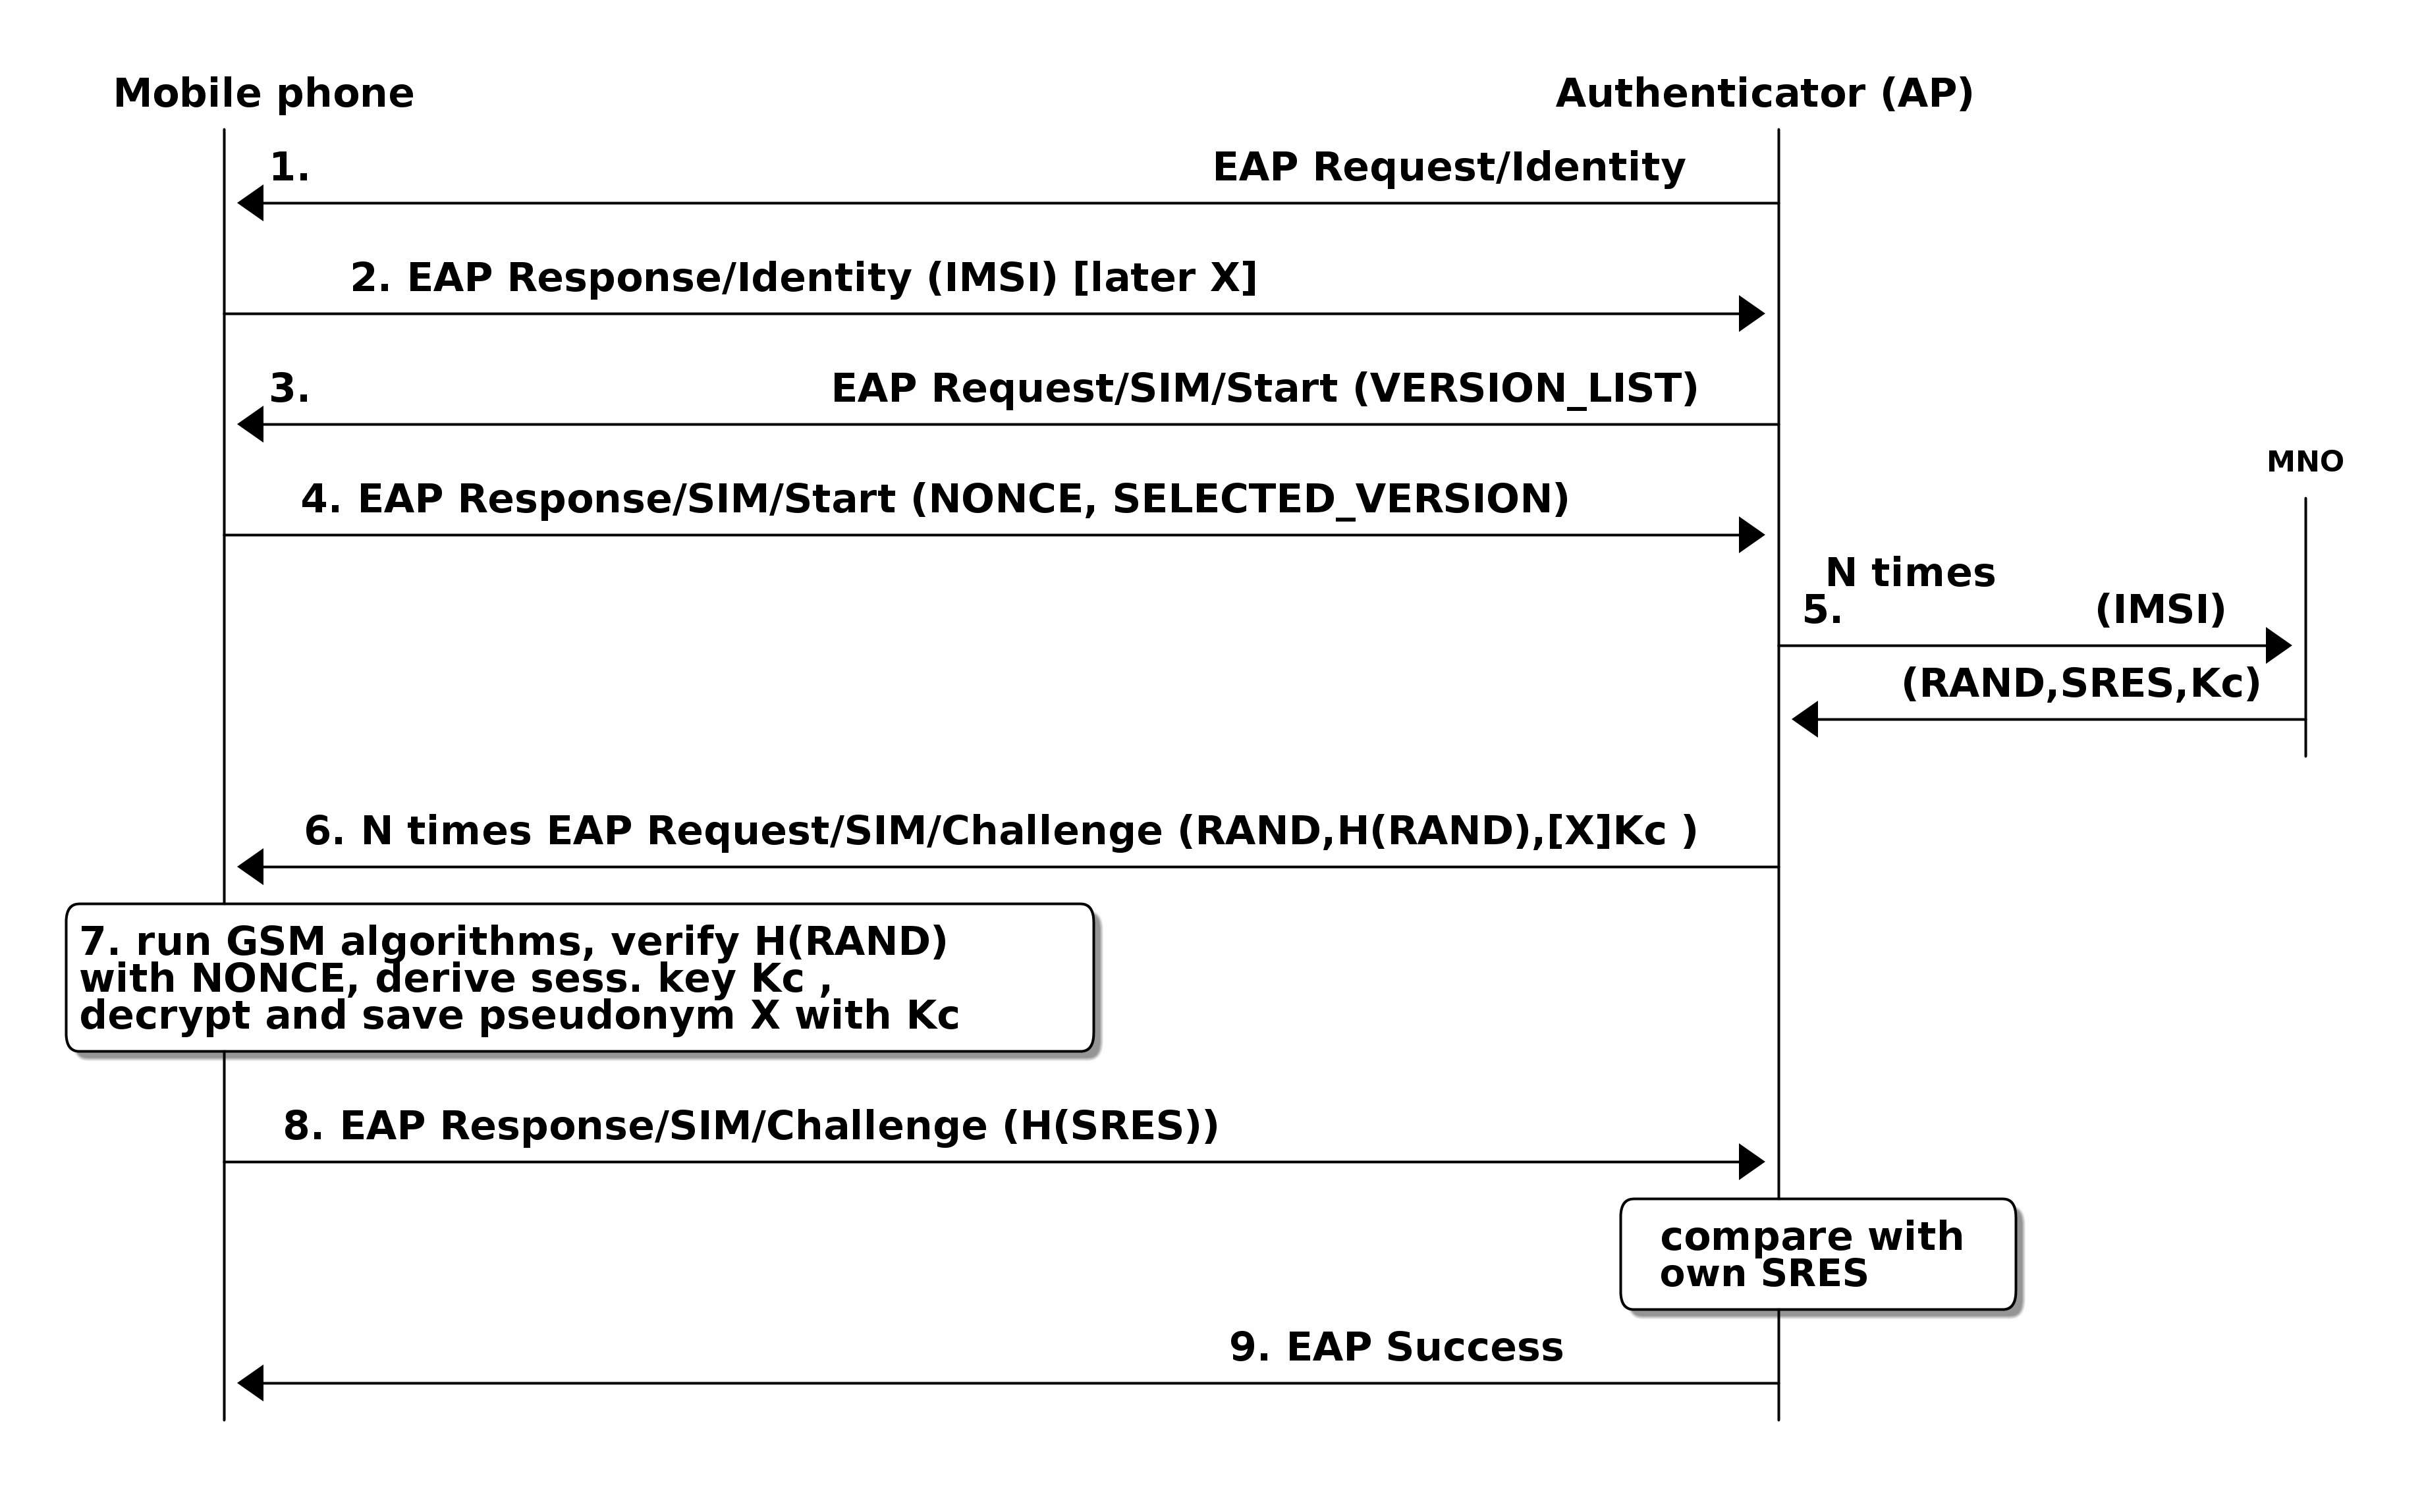
\includegraphics[width=.9\linewidth]{eap-sim-full.png}
\caption{\label{fig:eap-sim-full}EAP-SIM authentication sequence diagram, without RADIUS, based on RFC4186}
\end{figure}


\begin{figure}[htb]
\centering
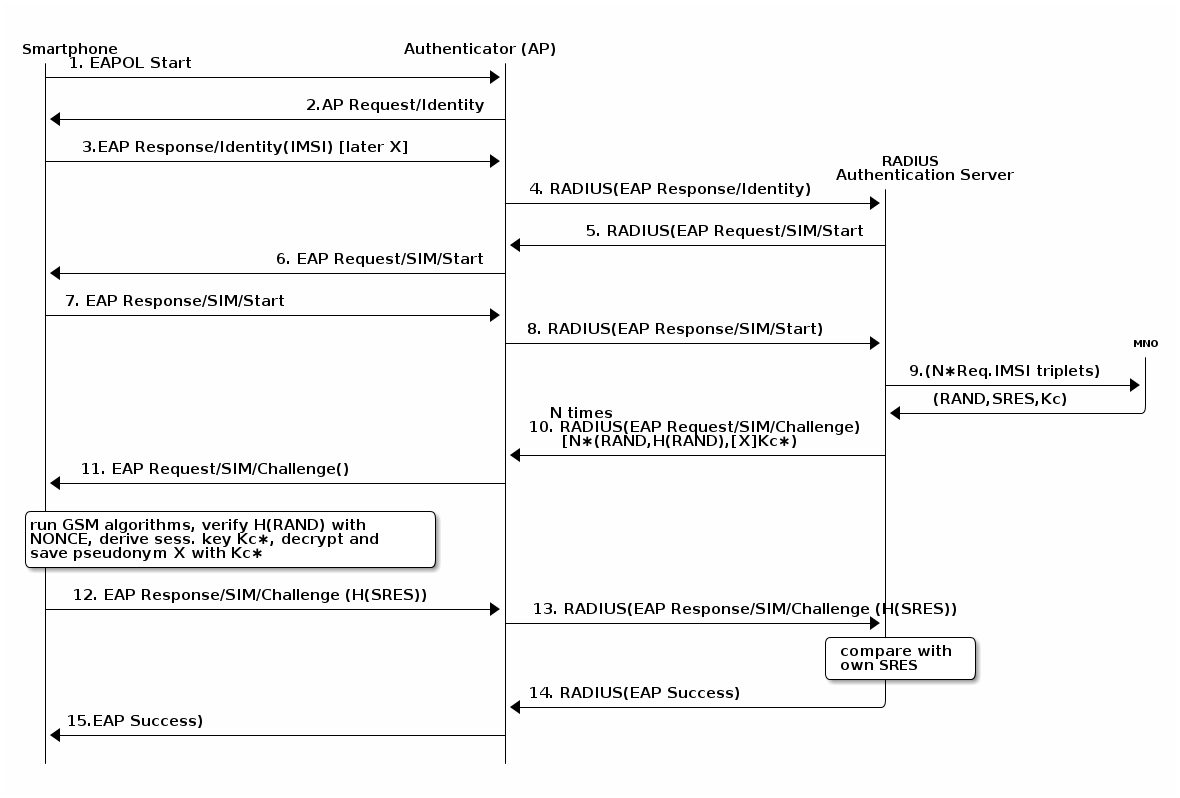
\includegraphics[width=.9\linewidth]{eap-sim-radius.png}
\caption{\label{fig:eap-sim-radius}EAP-SIM full authentication with RADIUS}
\end{figure}
\section{Trust}
\label{sec-2-6}

Secure communication has many layers and on its base lies trust. 
Only after completing trust setting phase it is meaningful to complete
the other security layers. For example, secret keys enable encrypted
communication, but they need to be delivered first through an trusted
channel. Same applies to exchanging public keys in PKI solution,
 and so it can be seen that trust really is the first layer to
be fixed.



Even without trust, some form of secure asymmetric key-exchange is achievable
with Diffie-Hellman key-exchange\cite{diffie1976new}. Unfortunately, it is vulnerable
to Man-in-the-middle(MitM) attacks, where protocol does not notice, 
if messaging goes through third party, which impersonates itself to 
both ends as being the corresponding messaging partner. MitM can
read and decrypt encrypted messages and forward possibly changed message with
correct looking signature.
With trust set between two devices, i.e.,  if they can securely
authenticate each other, secret communication is possible. 
Secure network configuration and credential exchange is then possible.


As mentioned earlier, the SIM and MNO trust each other hence mutual
authentication between them is possible and that is later shown to be
an important factor.  
Key distribution problem mentioned in Chapter\ref{cha:intro} is solved
already at SIM-card distribution phase. 

Now, how this trust could be used to include other components under
same trust circle in the homenet?  As AuthN-AuthZ at home proceeds
through Authenticator, maybe Authenticator can deliver this
information further and use it as a derivation function to extend
trust.

EAP-SIM derivatives provide strong AuthN which means here two-factor
AuthN. Software certificates, while stronger than regular passwords,
on the other hand do not possess the properties \emph{non-copiable} or
\emph{unique}, so they can only be considered as strong passwords and they
do not full-fill requirement for two-factor AuthN.  If we nonetheless
were using software certificates with method such as EAP-TLS, then the
certificates (for CA and client) and the private key should still be
provisioned first, which would defeat what we wanted to achieve.



\chapter{Managing Home Networks [or Home network architecture]}
\label{sec-3}
[ keep this security oriented, Forget sections \& subsections style.]

\section{Home network architecture and IETF}
\label{sec-3-1}


Home network is a computer network located at person's home. It consists
of devices and their connections, either wired or wireless.  This
thesis denotes home network as homenet, although the name 'homenet'
is reserved to Internet Engineering Task Force Working Group's (IETF
WG) homenet.
IETF is responsible for the most Internet technology standards and 
WG homenet was started in year 2011.
Current drive in homenet management is towards IPv6 environment
 as it allows future  addressing and routing needs. As old technology
cannot be forgotten, homenets will be heterogeneous having both
old and new technology, and their interoperatibility is important in
planning future homenets. Segmenting home in multiple subnets will belong
to homenets and will include areas for home members, guests,
and management.



Securing homenet and its router's configuration can be done for
example first limiting access to their administrative ports
with static or dynamic access control lists (ACL) in
routers. To get through administrative ports, i.e., to login and make
configuration changes, there exists either AAA or local authentication.
Authorized agents can then make changes, either direct in the device or through some
management protocol such as SNMP or NETCONF[source needed?].  SNMP has been in
use for over 30 years and is well supported in routers. Yet there are
multiple version for this protocol. While earlier versions (v1, v2)
did not provide any encryption of messages, version 3 knows for example
about public keys and is secure enough when used correctly.
NETCONF is\ldots{}


CPEs (Customer-Premises Equipment) such as ADSL broadband routers or
set-top boxes, connect customer's network to operators network.
Management of CPEs on the border of homenet and operator has 
been done already earlier.For example, TR-069 standard\cite{iptvtr069} for CPEs
has been used to implement self-configuration archi\-tecture in
home networks\cite{tr069rachidi2011}.


RFC7368 about IPv6 Home Networking Architecture Principles from
Arkko\cite{rfc7368} defines the borders of the homenet and states that
internal borders in homenet should possibly be automatically
discovered. Limiting those borders to specific
interface type makes it difficult to connect different realms locally.
The same document continues stating
that while homenet should self-configure and self-organize itself as
far as possible, self-configuring unintended devices should be
avoided and let homenet user decide whether device becomes trusted.
So, these statements reveal us that homenet environment still needs
external configuration even with the proposed automation aids.





Homenet WG proposes the use of Public Key Infrastructure (PKI) at the
home. The public key cryptography is processor intensive and its
asymmetric keys are usually used just in the beginning of
communication. There they can be used to securely negotiate symmetric
keys which allow faster cryptography processing.

To use PKI, bootstrapping protocols are first needed for trust
anchoring and AuthN.  Despite the etymology of name bootstrapping,
``Lift oneself by his own bootstraps'', bootstrapping usually needs
some input from outside.
For that Behringer's draft\cite{draft-behringer-bootstrap} proposes,
that first one device is chosen for the trust anchor and trust is
built upon that anchor. This anchor device then becomes homenet's
Certificate Authority (CA) service. In the end, rest of the homenet will be
imported into homenet through CA, which returns their certificate
requests signed.


Key creation, key exchange and their usage is explained in similar
draft from Pritikin\cite{draft-pritikin-bootstrap}. There is also discussion about using
manufacturer provided device certificates as trust anchor.  



This model could also be expanded to a full ticket enabled
Kerberos-style network, where time-limited tickets (tokens) exist for
both authentication and authorization for different services. Trusted
Third Party authentication center would be setup with the help of MNO.
One service would then authenticate an entity, here smartphone, and
give it a time-limited ticket as a proof that the entity has been authenticated.
When the entity wants to connect to the service, it asks from the central 
server again for ticket, but this time for the service by presenting
the authentication ticket. In return it receives a service ticket which
it can present to the wanted service. 
If EAP-SIM was applied in such environment, it would be used only once, namely in
the bootstrapping phase to setup the CA trust anchor.  






Homenet configuration itself is mostly excluded from this work.
For example, 
it is desirable, that changes in homenet are done only through
local controller, not at local device because of
synchronization issues, even 
if synchronizing algorithms such as Trickle\cite{rfc6206} are used in
homenet for code propagation. Configuration also includes configuring
power level setting of devices to save electricity based on usage
profile. For example at nights or when there is nobody home, some
devices do not need to be working at their maximum capacity. Instead,
we study interface of AAs.  Main points here are an existing
infrastructure (phones, internet access, Wi-Fi access points),  a strong
authentication (two-factor), and existing authentication methods
(EAP-SIM, EAP-AKA, EAP-AKA').
\section{Centralization trends in management}
\label{sec-3-2}

Traditionally, management of network devices has been done
individually using each device's console or web-access.  As the number of
devices has increased, it would have been reasonable to rationalize
the process by utilizing a central management, not least to prevent human
errors for repetitive tasks.  Yet, at home, network devices often are
too heterogeneous, bought at different times from different vendors
and so incompatible with each other to fully benefit from
centralization. 

To help moving the management to a more centralized
model, smartphone is set here as a central managing local
controller.
Usually, home users already have a phone, which can be considered as
`smart'. Most smartphones have Wi-Fi capabilities and writing programs
for them is possible even with only little knowledge.
When we choose a smartphone to be the management point, the other benefits are
numerous:  a management software can be delivered and
updated from cloud to diverse smartphone types, existing user
base having smartphones is enormous, and as the most important fact, the trust anchor can be set to the smartphone.

The users are located in operators' user databases
in Home Location Registry Authentication Center (HLR-AuC), which still has orders of
magnitude more users available than any other organization. 


\chapter{Design of home network trust anchor and separation of change management}
\label{sec-4}




[Chapters contents here]
So, we need to change the management paradigm to central configured
model, bridge homenet to that model with a local controller 
and resolve the  work-flow of change management.







The smartphone connects with a Wi-Fi link to an access point (AP) in
 the homenet.  AP functions there as an Authenticator.  The smartphone
 and the AP must trust each other.
For the configuration\ldots{}
The smartphone will approve changes for homenet and is part of bootstrapping
new infrastructure. 

\section{Alternative methods for introducing trust anchor into the homenet}
\label{sec-4-1}

Before fully explaining our chosen method, we introduce some
alternative approaches for a trust anchor. The trust anchor is part of
bootstrapping. Trust information, may it then be a secret or some
other evidence, can be delivered to a trust device via physical
transport channel separate from the actual communicating channel.
Traditional way to do that is with a password inside a sealed
envelope or a one-time password list that for example online banks 
use today. The secret can also be sent as an SMS.

Trust can also be requested with the help of (upcoming) trust anchor's
unique properties. Recently there has been devices on the market that
have vendor certificates inside them[cite] which brings public key
infrastructure as one possible alternative.  The device proves its
identity by presenting a certificate, which has been issued by a
trusted vendor.  Private keys are in the device's trusted hardware
store.  Vendor-trust is needed for checking the issued certificates
and so the trust verification is merely transferred from individual
devices to trust verification of the vendor.  Root CAs are trust anchors
also and can in the same way be read from the device's read-only store.
CPE could use vendor issued certificate for AuthN of some earlier
unknown device.  If keys are stored in SIM as here, external operator
support is needed.


[Picture]

Other techniques  to use SIM's unique properties besides EAP-SIM
are for example Bluetooth SIM Access Profile(Bluetooth  SAP), 
direct connection through PC/SC (Personal\-Computer/Smart\- Card),
CallerID service from phone network, and
Mobile signature service such as ``Mobiilivarmenne'' in Finland.



Bluetooth SIM and PC/SC would need patching of smartphone's software
to work.  On the other hand, the smartphone would any way need to
download  a controlling application
in the beginning for advanced use, so these techniques could be
studied further in another work.

Caller ID as an authentication method uses GSM network's controlling
channels. When a phone makes a call, the receiving end gets 
to know callers phone number (IMSI) before it answers the call.
That information is called Caller ID and it has been in use
successfully for some door locking implementations. 
It does not cost anything for caller or responder,
because after receiving the CallerID  information, responder can hang
up upcoming call and no call expenses are created.
 It can also be made safe at least in Finland
by limiting which tele operators are allowed to connect.
















European Telecommunications Standards Institute (ETSI) defined a
standard for mobile signature services (MSS) in ETSI TS 102 204.
MNO's in Finland have implemented this as a 
service called ``Mobiilivarmenne``. 
For example, MNO Sonera's brand for  it is ``Sonera ID'' while MNO Elisa calls it
``Elisa Mobiilivarmenne''.

When AuthN and AuthZ comes from outside, one possibility is to use a
federated Mobile AuthN Service, which then is connected to MSSP(Mobile
Signature Service Provider) with ETSI-204. Benefits for ETSI-204
federation is that no single home device must implement it at home,
but also MNO sees service as just one client.  Without federation,
mobile AuthN services would need to be multiplied with number of the
separate homenets, which need authentication service.



Project Moonshot, if worked and used together with MSSP, may offer
SIM-based SSH-access to Authenticator. Modifications are then needed 
both in SSH server and client. Additionally EAP must be used through
tunneling, for example as an inner protocol of EAP-TTLS.\cite{moonshot}

At this point question might rise, why these external service
providers are needed. Is it not easier and simpler to just send 
an SMS with password code to the smartphone, when access confirmation is needed?
Mobile SIM provides two-way AuthN part as discussed earlier.l
Without need for strong AuthN, that model would indeed be 
simpler, but using SIM also solves initial key distribution problem.
Additionally, mutual AuthN problem would still need to be solved:
Who sent that password?



All this time it is assumed, that hardware does not lie. In case
the hardware has been tampered, we could not trust it and its claims.
For example, there have been attacks against SIM to reveal its private
key after SIM have been copied.  To verify, that a device has not been
tampered, a method called attestation can be used.
A device which has attestation capability such as 
hardware certificates or Trusted Platform Module (TPM) technology
can function as a trust anchor.
Such a device could be sent direct to customer with pre-configured
secrets and methods to take a place as a trust anchor. 
That leads us again to the key distribution problem.

There is also fraudulent Authenticator problem: the Authenticator may present some 
information to the Authentication server and other to the EAP-peer.
Mitigation for that is, that EAP-peer includes some 
characteristics of the Authenticator inside its EAP-message, which
then the Authentication server verifies (RFC6677)\cite{rfc6677}.



The phone brings trust to the homenet by completing full EAP-SIM AuthN through
the local Authenticator. SIM's identity is verified by HLR AuC at the phone
operator's end. The verification leaves a trail on the local Authenticator and
opens a trust channel for a limited period of time for changes from the phone.
[This was the most important paragraph of whole work. Thanks for
reading it.]





Requirement for homenet can be as small as having WPA2 Enterprise capable
AP. Almost any AP will do, but as an exception, cable modem Bewan, which 
has been distributed to many homes from the cable modem operator Elisa, was found to have only WPA2-PSK mode.
Additionally, managing user's SIM-card has to be registered as an admin user in homenet 
configuration, i.e. IMSI must belong to the admin group.
In this implementation, no extra application is needed in smartphone
for primitive trust, but later for more serious use some application is needed.
For added functionality, for example for logging admins out, OpenWRT
based software can be used, although those functions have not yet been
implemented. Disconnection issues are explained in Section
\ref{sec:disconnections}.

\section{Flow of design (already above)}
\label{sec-4-2}

Wanted: 
\begin{itemize}
\item separate MGMT net exists
\item SIM authentication to MGMT net is proven
\item changes are authorized if they come from MGMT net
\item log-out from MGMT net
\end{itemize}
(- spare connection, if internet link down)
(- fast-reauth, without MNO

Implications are, that when someone has access to MGMT channel,
everything is permitted. No security limiting as default 

[Basically 2. and 3. is like traditional corporate network with firewall.]

a. AuthN is proven

b. AuthZ decision has challenges

c. Change approving has three cases:
\begin{enumerate}
\item Changes are allowed, when port is open
\item Confirmation message from MGMT-net authorizes changes.
Message must belong to configuration and can be example a digested signature.
\item FULL: changes may come only from MGMT net.
\end{enumerate}


Use-case for adding admin user:

Let's first suppose, for case of simplicity, that the homenet has been
already configured(bootstrapped) and it is functioning properly.  The
home configuration model has been copied[inserted, etc] to the cloud.
When changes are made to the cloud model through authorized cloud
administrator users (operators), those changes are later also committed
in to the production in homenet. There is no magic here, plain
configuration change, just this time externally initiated.

Now, let's think what happens, when the cloud operator (or owner of
homenet) tries to modify attributes, which give access to new actors,
such as new operators, who would want to have access to separate
segments of homenet.  First we need to have that segment separation
change approved and after that we want to allow the newcomer account
to have access to that segment and only to that. For the first part,
which is normal operation, approving would perhaps yet not be
necessary, but for the second part we need some checking unless our
trust to cloud operator is ultimate.  [FOR approval needs, discuss
this with the team.]




When CPE of homenet is about to input configuration changes which
would change balance of authors or roles (if role-based authorization
in use), it needs to check if that is permitted.  Permission would 
need to be asked from trusted point, here mobile SIM but instead of
that the CPE checks from its state database, 
whether mobile SIM has been given access to management network.


CPE wants to verify, if the changes are authorized. They are, if currently
smartphone user is logged in management network (i.e. management is allowed).



Alternative method is that the changes could be marked some way, so that they need
approving and then there could be a specific change-approval message,
which must be sent through management network, perhaps including digest
of change message as a verification.

Because smartphone is not actively listening the CPE, how it could
input that request? 

There are three planned ways to distribute changes.

\begin{enumerate}
\item Changes are delivered normally from cloud to CPE (CPEs) without
interaction from the smartphone. Such changes would not need
AA at all or changes include credentials to login to targets.

\item Changes are delivered from cloud to CPE functioning as a central
management station without interaction from the smartphone.  Digest
of what is going to happen would be sent to smartphone from BaaS
over the air (OtA). Smartphone would authenticate in to management
network (if not already there) and send through it the digest token
it received from cloud as an approval message to central management
station inside homenet, which then forwards configuration changes
to other devices.

\item Changes are delivered from cloud to smartphone, which after
authenticating into management net, forwards them through management
net to each and all devices.
\end{enumerate}


The smartphone may receive the authentication token with 
a message explaining what is going to happen in the change.
As the CPE and the Authenticator may be separate devices, approving
happens by sending the token from the smartphone to the CPE via the
management network where the Authenticator gives access.

It must be noted, that the smartphone can already have an association
to a non-management network with Wi-Fi. If that is the case, it first
must disconnect from there and then connect (i.e. AA) to the correct management
network. That implies disconnection from other services using Wi-Fi
link, because smartphones currently have only one Wi-Fi radio
available and routing prefers Wi-Fi as a default gateway, although
possible 3G data link still may stay operational.


\section{Chosen design and why (Rationale)}
\label{sec-4-3}
\label{sec:chosendesign}   
Network can be divided into separate segments. 
First, there is normal access network which provides
connectivity. Second, there is network through which devices are
managed, so each device need to have at least two connections: one for
access and one for management. It is not defined, if those connections
are physical or virtual (VLAN's etc). 
Analogy to real world would be public access corridors and doors for
customers separate from privileged doors for service personnel.

Access to the network segments is checked in routers with access control lists
(ACL), where decision is made based on current configuration or user's
role.  Once user has been authorized into management network, access
stays open for him, at least for a (predefined) limited time.

So, instead of checking user's credentials each time data is received
this model only checks, from where data is received. 
Data received from the management network is granted for changes.
It is arguable a lighter method than always
fully AuthN and AuthZ but may suffice here, at first.

Naturally one will first challenge the solution, if
management network is thought to be in secured zone.
but sure devices have additional protection for logging in them. 


Example of a complex solution would be a traditional firewall and packet
inspection in the interconnects. Even more complex would be that traffic
always travels through Access Control Engine such as Google's
BeyondCorp \cite{2014-beyondcorp}, where all
traffic is suspected as being external, even when it originates from inside networks.


In production, some changes in local controller are propagated to homenet
via management network without need for an extra authentication phase.
The local controller does not interact there. An example of change is
a modification in network segment, which does not change network topology of other domains.
Those changes or alternatively changes that do need authorization
should be enumerated, which ever would be smaller set.  

In our model, only initial bootstrap needs the authentication with
smartphone as well as change of admin roles and some dangerous
combination of commands.

[ sync. part to misc Section ?]





When homenet needs secure binding to the smartphone, earlier
mentioned trust is the first one needed.  The trust is achieved by
checking whether the smartphone can access home management
network using only its trusted SIM-card, which provides AuthN. AuthZ in
turn is compared to existing roles of IMSI in the Authenticator.


[This has been explained in 802.1X Section in the begin. TBD]

Technically we use in Wi-Fi connection IEEE 802.11i (also known as WPA2), which includes
802.1X as port based access protocol.  802.11i defines there
authentication, authorization, and cryptography key agreement.
 It uses EAP for selecting authentication 
mechanism, after Authenticator requests smartphone to identify itself as in Figure xxx is shown
Messages are carried over 802.1X or RADIUS depending on transport
medium as of Figure\ref{fig:eap-layers}.


When AP forwards authentication request to next RADIUS server, it can
ask or receive, beside AuthN and AuthZ, other service parameters, such
as provisioning. That would allow the smartphone to connect to
specific management network access either via CLI or SNMP or similar
 \cite[p.4]{rfc5608}.  RADIUS can carry extra attributes in its
ACCESS-ACCEPT message.   In essence, AuthZ part itself can be thought as
one type of service provisioning. 


There exists RADIUS attribute types for directing user into specific
VLAN. If those do not suffice, there is also special Vendor Specified
Attributes (VSA). VSAs allow vendors to define up to 255 own
attributes that can be used in provisioning in homogeneous environment. 


That way (3rd party) Authentication server can decide which network
segment the device would be put.  In our case, admin users are put in
to the management network.  Yet, usually RADIUS ACCESS-ACCEPT message,
which means AuthN and AuthZ were successful,  puts the user in
default network, i.e., just gives it basic access. As for other
provisioning parameters, not all end devices support them.

In the first prototype it is enough to identify authorized
smartphone's SIM.  Smartphone holding the SIM is granted the access to
the parts of the management network and is authenticated strong.  User
management is outsourced to Mobile Network Operator(MNO), which
already has provided SIM cards to users. What remains, is the adding
of the user's IMSI to the authorized users' list. That list can be
located on diverse place, as can be seen in xxx


After authentication and authorization has succeeded, session key
creation occurs (WPA2 session) between AP and the smartphone. 
The Authenticator has opened port to the smartphone for
configuration changes. 
The Local RADIUS (if existing) has trails of successful
authentication and knows which IMSI has successfully authenticated in
the home net. It also knows mapping between IMSI and temporal IMSI for
cases where the smartphone later would need  re-authentication.



\section{[Need for Security bootstrapping]}
\label{sec-4-4}
[removed, NOT YET trust anchor methods HERE!!! ]



[Description of General Bootstrapping architecture (GBA) vs. yet
another custom architecture. Maybe parts of architecture
such as using SIM-auth (EAP-SIM) or CallerID, how they differ. 
What is needed? How GBA could be used here?]


In Behringers work-in-progress  bootstrapping \cite{draft-behringer-bootstrap},
AuthZ happens likewise first at cloud provider's
end, but after checking device's Vendor certificates, cloud provider
gives device a ticket of authorization like in Needham-Schröder or
Kerberos implementations. Device presents that ticket to CPE which
finally can decide, whether it allows change. 
Instead, here the Authentication server can be external RADIUS server,
but usually the final decision point lies at the Authenticator in CPE.


\section{Access methods to Wi-Fi with only one SSID}
\label{sec-4-5}

[To be cleaned!]

Today, homenets usually consists of only one Service Set ID (SSID)
Wi-Fi network though it is possible to define multiple SSIDs in
an access point. Having multiple SSIDs enable us to dedicate one of them
to management network. 
To enable EAP-SIM method, it is necessary to use WPA2-Enterprise mode
an as such, to use RADIUS server.

It was not found, how Authenticator could use the same network with
both WPA2-PSK (or open access) and WPA2-Enterprise, so
separate SSID for management network was technically needed.
If Wi-Fi was limited to only have one SSID, then we would need another
way to separate access requests to management net.  Access to Wi-Fi
can be separated by multiple realms (different username domains),
different authentication methods, or user's role
given by Authentication server. Management through Wi-Fi has then three
options.  Without RADIUS, access is open and the only checking comes
from the used management protocol and its access control.

[2015/05/11 NEW! This must be told everywhere, devices still have their own access
control! Or do they use RADIUS? Now RADIUS is used to carry on EAP auth to get into access
network, why not use it also to get in device? ]

With WPA2, PSK is used, but no EAP or RADIUS as backend.  With EAP,
RADIUS server is the one who returns correct values to get in
management network in ACCESS-ACCEPT message as was
explained in Section \ref{sec:chosendesign}.


\subsection{HS2.0 [If deleted, remember also from conclusion! TBD]}
\label{sec-4-5-1}

Wi-Fi Alliance has certification program (Passpoint) for Hotspot2.0 compatible
devices.  Hotspot 2.0 enables selection of network based on ownership,
services and performance characteristics \emph{before} Wi-Fi client has
been associated to Hotspot 2.0 AP. The technology is built on
IEEE 802.11u specification.




It is well known, that usability of Kiosk-mode Wi-Fi
 networks is burden, because user needs to go through 
web portal logins with username-password authentication 
procedure and those are different for every network.
HS2.0 would help there.

In 
\url{http://www.ericsson.com/res/thecompany/docs/publications/ericsson_review/2012/er-seamless-wi-fi-roaming.pdf}
goals are to smooth roaming between Wi-Fi and 3GPP/LTE networks
and bring operator-grade to Wi-Fi by putting control in operators side. More
than offloading traffic, plans are to bring other services also to Wi-Fi.

TO DO: check 802.11u features and what they add to 802.11-2007
\begin{itemize}
\item interworking with ext networks
\item hs2.0 is extended 802.11u
\item next generation Hotspot
\item advertises external networks \emph{before} association. no need to
select Service Set ID (SSID)
\item access network type, roaming consortium support and venue information
\item some QoS mapping
\item emergency services (not in HS2.0)
\end{itemize}


\section{Scenarios for authorization (AuthZ)}
\label{sec-4-6}

[Place of Authorization decision  ]

AuthZ decision usually happens at home.
If the decision is made on remote AuthN server, 3rd party, 
then that server needs to have access to 
cloud service's AuthZ data. 
Further it seems inevitable, that just like the homenet model
having AuthZ data of eligible IMSI accounts is in the cloud, 
then also delegating AuthZ to cloud would simplify homenet
functions. Instead of putting logic on CPE for AuthZ, CPE
could just trust the 3rd party service's AuthZ message, which is 
RADIUS message of either \emph{ACCESS-ACCEPT} or \emph{ACCESS-REJECT}.


Here are presented 5 scenarios for possible locations of AuthN and 
AuthZ points. Authenticator is the entity which gives the final decision 
about access. In most cases it is located in the
local AP, but it can also be external, like in scenario V in 
table \ref{table-scenarios}, where locations for Authenticator (AA),
AuthN, and AuthZ are marked as (I) for internal or (E) for external.

\begin{table}[htb]
\caption{\label{table-scenarios}Location of AA, AuthN and AuthZ in scenarios I-V}
\centering
\begin{tabular}{llll}
scene.no: & AA & AuthN & AuthZ\\
\hline
I & I & E & E\\
II & I & E & I\\
III & E & E & E\\
IV & I & E & E\footnotemark\\
V & - & - & -\\
\end{tabular}
\end{table}\footnotetext[1]{BaaS provides}


\label{scenario-i}
The first AA-scenario is presented here thoroughly as an example.
The goal is to make trusted configuration change. 
The steps are numbered in Figure\ref{fig:scenario-I}.
Configuration change is allowed, if CPE gets ACCEPT from MNO.  MNO gets
information of allowed users from Cloud (BaaS [def.])


\begin{figure}[htb]
\centering
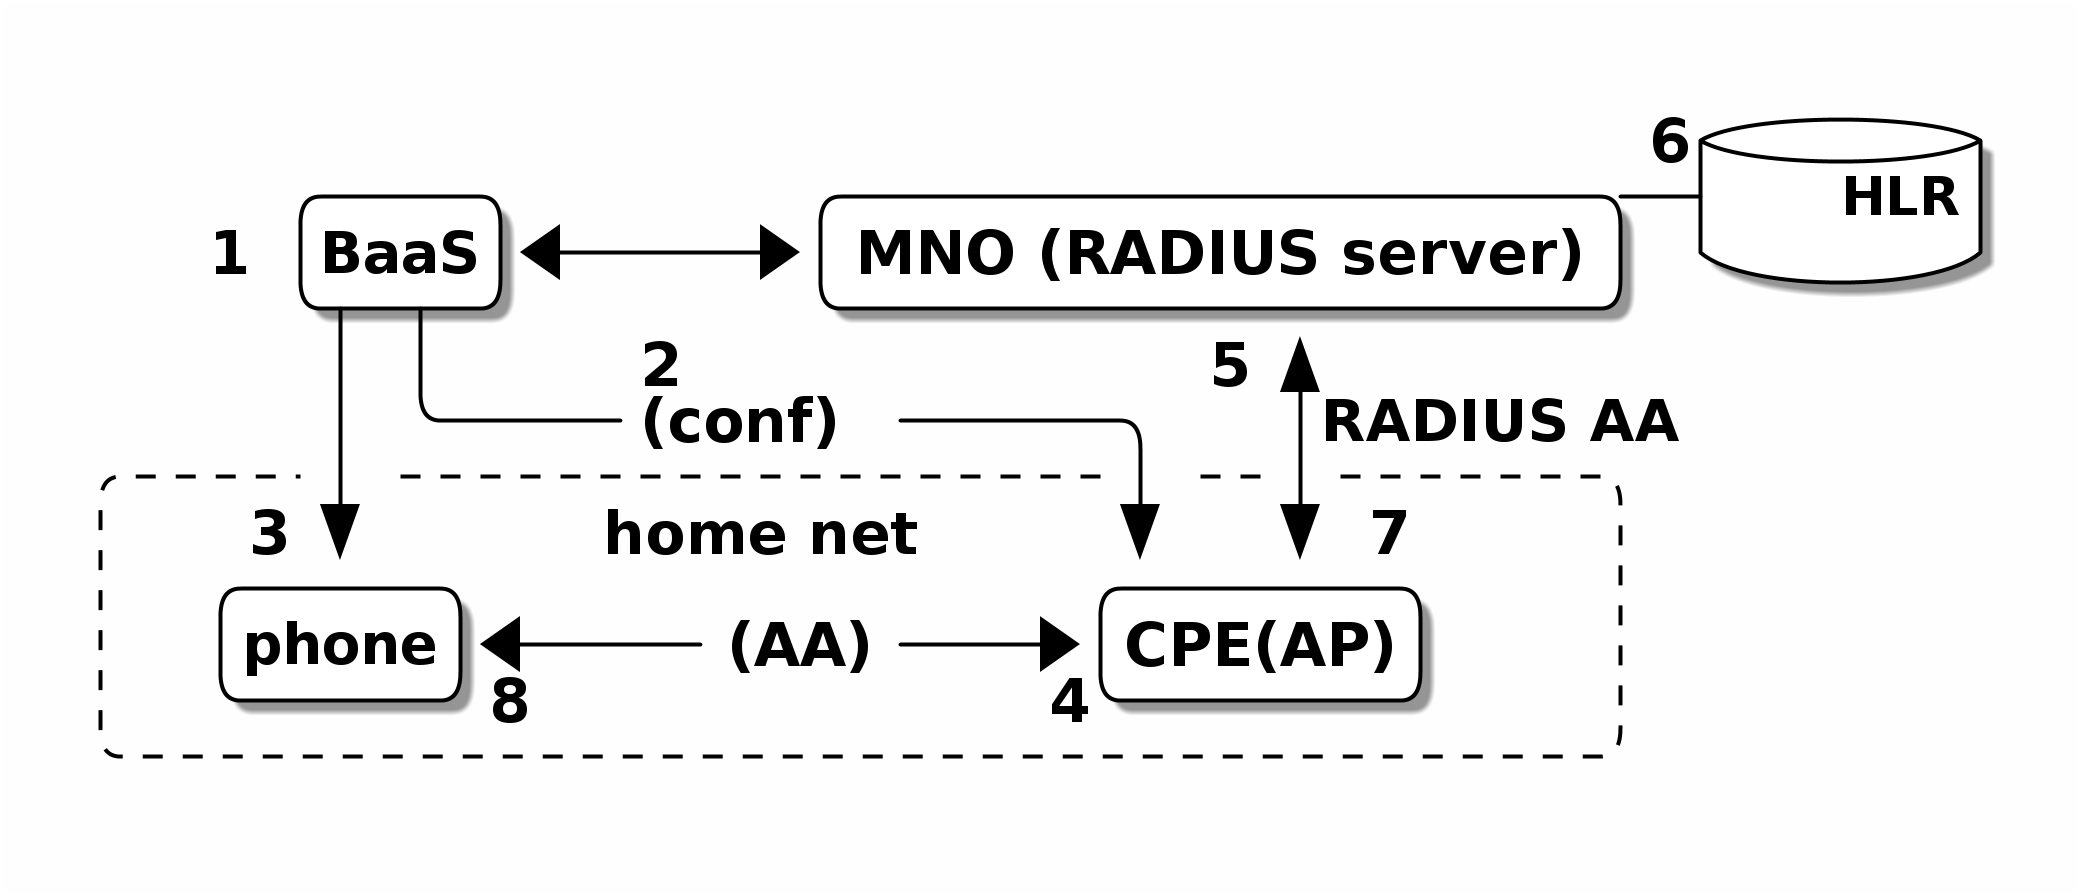
\includegraphics[width=.9\linewidth]{scenI.png}
\caption{\label{fig:scenario-I}Scenario I with 3 separate domains: BaaS, MNO and homenet}
\end{figure}

[ Maybe replace BaaS with CLOUD] 


[ alt. presentation of flow number I, list ] 

\begin{enumerate}
\item The model has been changed in the BaaS (1).
\item BaaS send changes to CPE (2).
\item If changes are privileged, they need to be approved by phone user.
Changes are sent also to the phone(3) and phone user must authenticate
itself to the management network.
\item Phone user starts authentication process to management
network using EAP-SIM and reveals its IMSI(4).
\item CPE  (AP) forwards authentication to MNO's RADIUS server with
RADIUS protocol (5).
\item MNO have RADIUS server running and it authenticates IMSI user with
  its HLR-AuC (6).
MNO also asks from BaaS, whether IMSI user has admin-role (AuthZ). [how long does it take to ask?]
MNO returns in RADIUS message either \emph{ACCESS-ACCEPT}, if user is both known AND has admin role 
  or \emph{ACCESS-REJECT} (7).
\item CPE receives this ACCEPT or REJECT. If there were other RADIUSes
between CPE and MNO, they would have acted
as proxy RADIUS servers.
\item IF ACCEPTed, then mobile is both authenticated and authorized (8) and
can send configuration change message to CPE, which recognizes it
coming from authentication network.
\end{enumerate}



[ alt. presentation of flow number II, paragraph ] 

The model has been changed in the BaaS (1). BaaS send changes to CPE
(2).  If changes are privileged, they need to be approved by phone
user.  Changes are sent also to the phone(3) and phone user must
authenticate itself to the management network.  Phone user starts
authentication process to management network using EAP-SIM and reveals
its IMSI(4).  CPE (AP) forwards authentication to MNO's RADIUS server
with RADIUS protocol (5).  MNO have RADIUS server running and it
authenticates IMSI user with its HLR-AuC (6).  MNO also asks from
BaaS, whether IMSI user has admin-role (AuthZ). [how long does it take
to ask?]  MNO returns in RADIUS message either \emph{ACCESS-ACCEPT}, if
user is both known AND has admin role or \emph{ACCESS-REJECT} (7).  CPE
receives this ACCEPT or REJECT. If there were other RADIUSes between
CPE and MNO, they would have acted as proxy RADIUS servers.  IF
ACCEPTed, then mobile is both authenticated and authorized (8) and can
send configuration change message to CPE, which recognizes it coming
from authentication network.

While changes has been already sent to CPE direct and only let it
wait for approval, then when CPE receives ACCESS-ACCEPT, it could
already proceed on propagating those
changes.  Otherwise, after certain timeout, CPE must stop waiting
for phone's approval and drop changes. [this was the question
somewhere, ``triggering'']


This simplification has pitfalls. If mobile stays in management
network continuously, how are upcoming changes separated? Mobile should
either be dropped out from management network right away after changes or
after predefined timeout period.  If on the other hand, mobile must
send changes itself, then it would be possible that access in the
management network has short period of time, when phone 
holds that status or acceptance token. For example for 10 minutes connection
would be open for changes. Then changes would not go directly to CPE
but instead to , but they would include some token to phone, which is
needed for approval message.


\label{scenario-ii}

In second scenario (Figure\ref{fig:scenario-II}), AuthN is asked from MNO but
AuthZ is checked from local database. Local data comes from data model
i.e. from configuration data and will be saved in CPE, or some other
place within homenet.


\begin{figure}[htb]
\centering
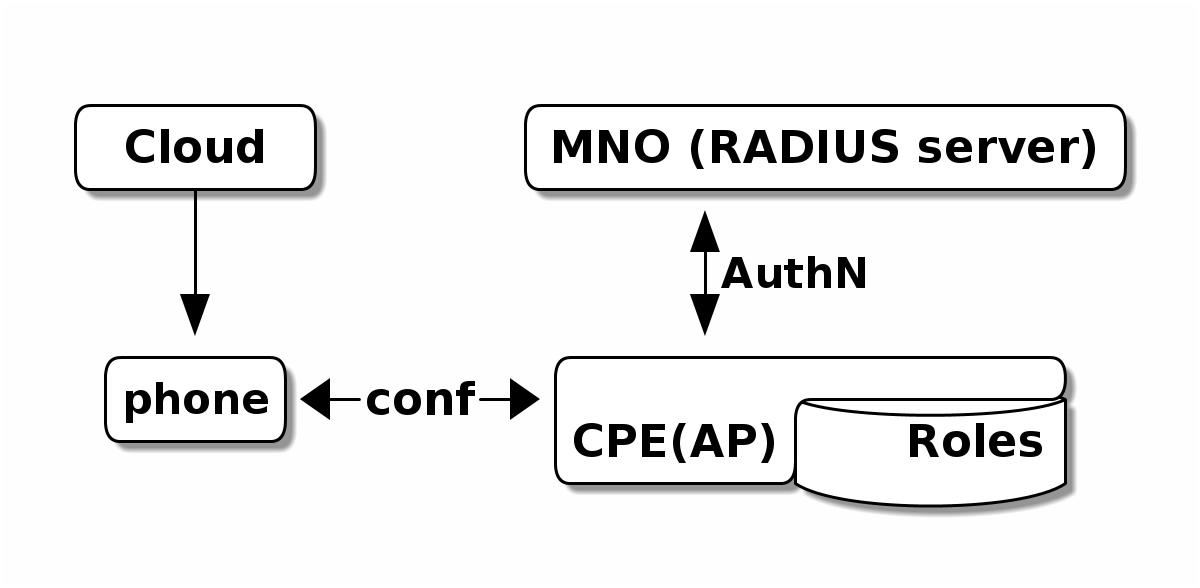
\includegraphics[width=.9\linewidth]{scenII.png}
\caption{\label{fig:scenario-II}Scenario II with AuthZ in homenet}
\end{figure}


\label{scenario-iii}

Similar to first scenario is scenario III (Figure\ref{fig:scenario-III}), 
but this time there is SP between CPE and MNO, so AA is fully outsourced:
local AP communicates with RADIUS protocol to the external
Authentication server. That in turn gets AuthN from MNO via its
hlr-auc-gateway and AuthZ from BaaS.
Locally there is a cache for roles in case of network disconnectivity.

Here benefit is, that 3rd party Authentication server may have direct
contracts to many MNOs, so user does not need to find and choose
them. As a bonus,  MNOs already delegate requests to right operator, if
they happen to get AuthN request which does not belong to them.
This is similar to federated service.

\begin{figure}[htb]
\centering
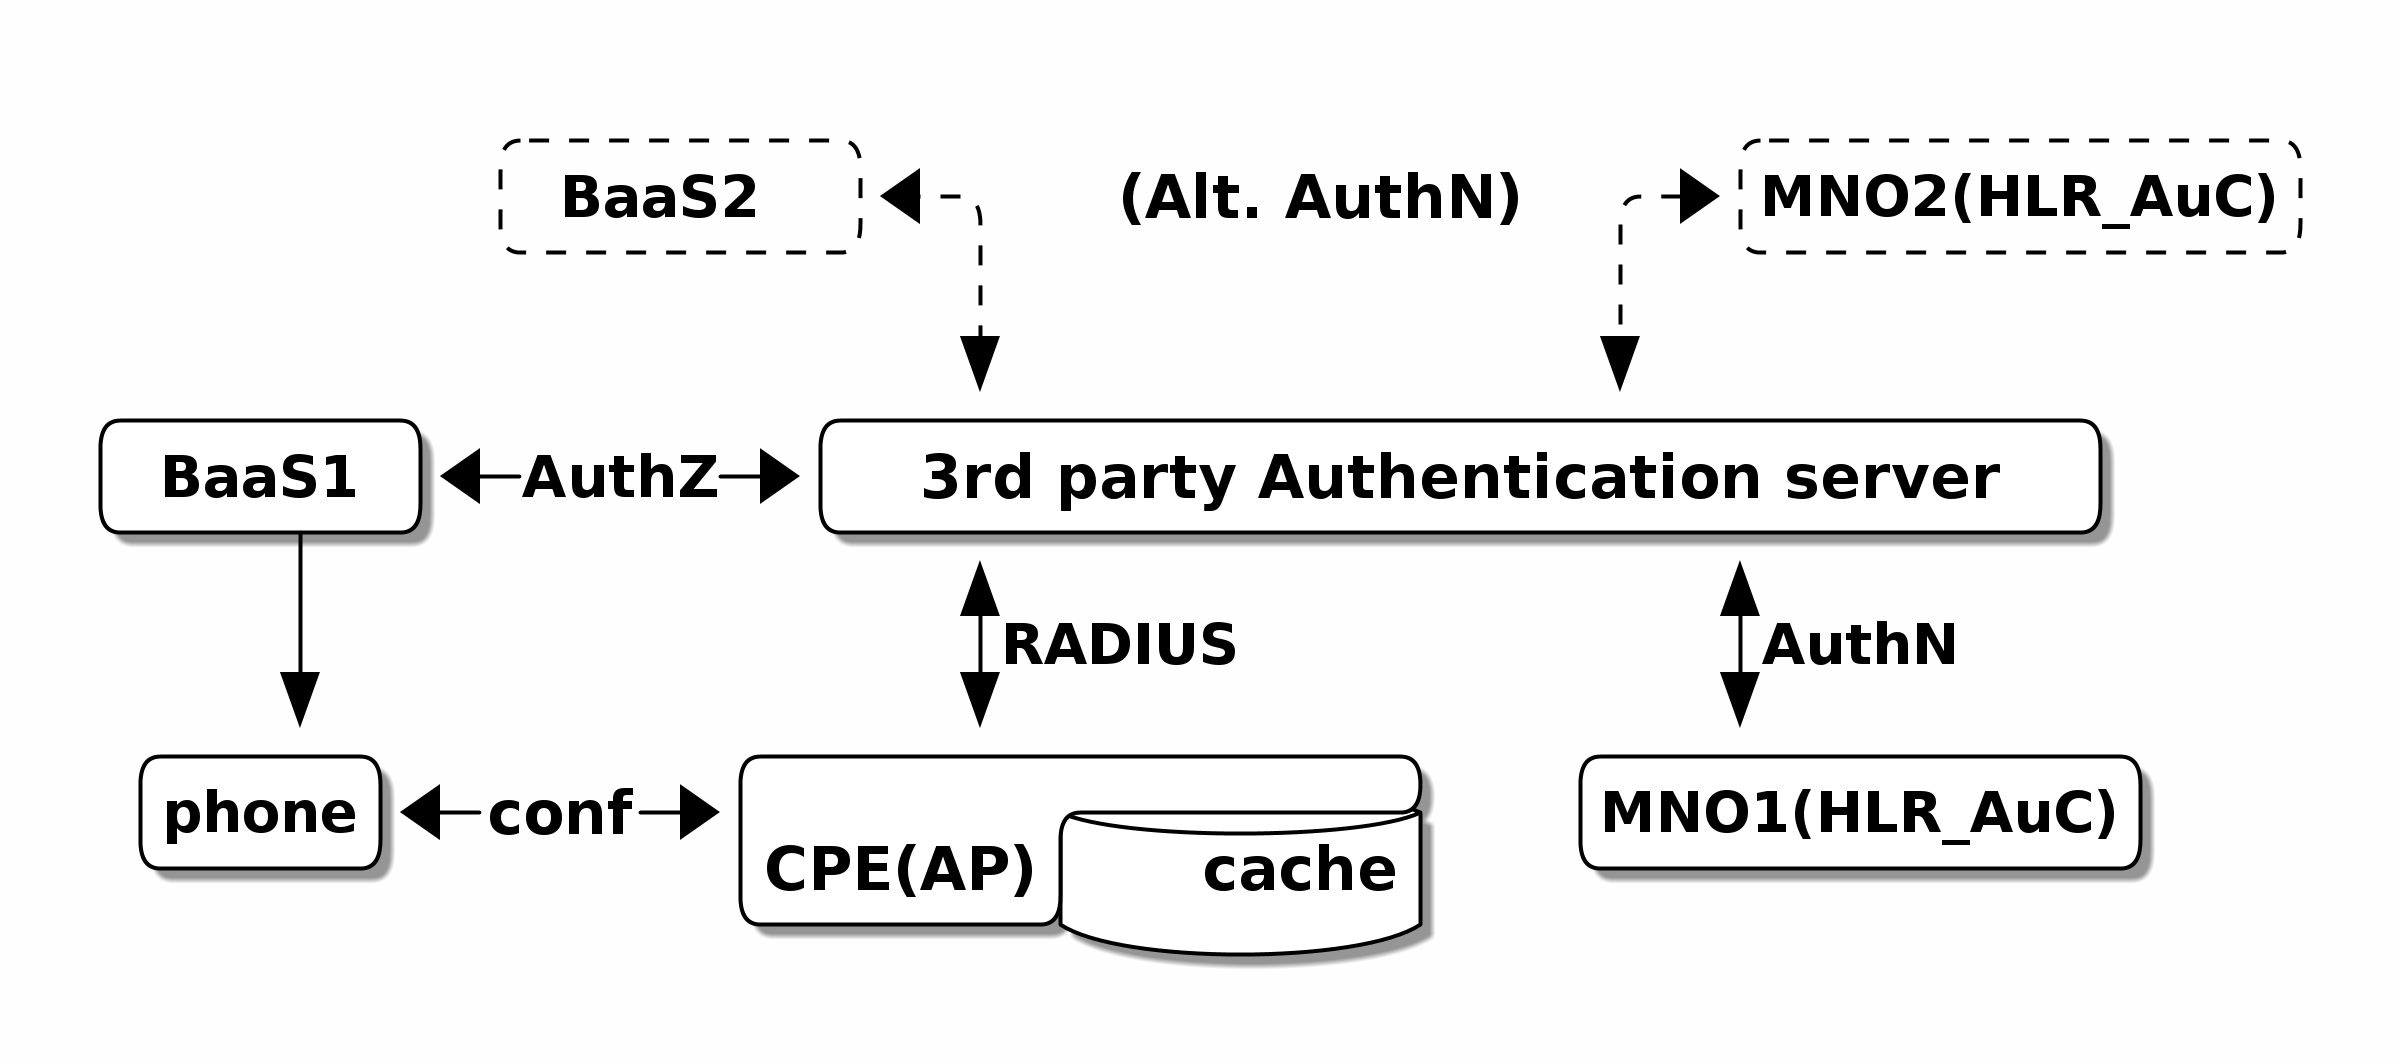
\includegraphics[width=.9\linewidth]{scenIII.png}
\caption{\label{fig:scenario-III}Scenario III with outsourced AA}
\end{figure}

Allowed users are verified from BaaS's registries and specific IMSI is
authenticated from MNO.  It may need some preparation, if SIM
identities are temporary i.e. TMSI is used.  Still, IMSI is carried out at first message
of full authentication. Later, the server would need to have mapping
between IMSI and TMSI, but because only full-authentication is used,
there should be no problem.


\label{scenario-iv} 


Scenario IV (Figure\texttt{fig:scenario-IV)} is almost like scenario II, but
AuthZ is always checked from BaaS. If there are no connection to
cloud, fall-back is to work as II. So also this scenario needs local
store for admin IMSIs.

\begin{figure}[htb]
\centering
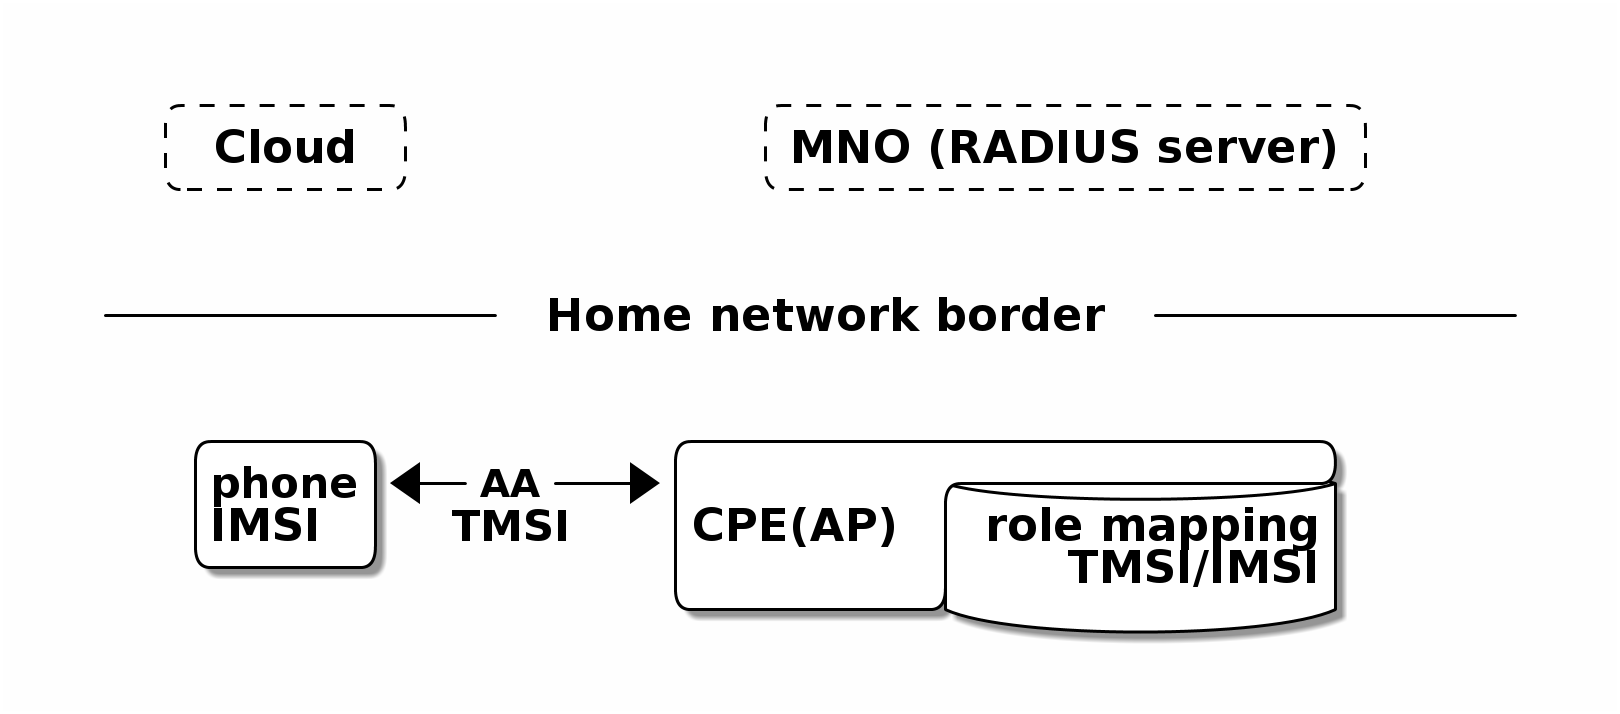
\includegraphics[width=.9\linewidth]{scenIV.png}
\caption{\label{fig:scenario-IV}Scenario IV, AuthZ from BaaS, AuthN from homenet}
\end{figure}

In the last scenario (no figure), nothing has yet been configured. The bootstrapping
is not done yet. The scenario can be any of I-IV, but no trust nor roles are present in CPE.
\section{Ways to modify RADIUS messages [perhaps to security integrity chapter?]}
\label{sec-4-7}
\label{sec:radius-macs}
RADIUS messages are not protected from eavesdropping, but they have
integrity fields to notice if tampering has been done.  
Integrity field is called a Message Authenticator.
Notice the use of the term \emph{Authenticator} in different context here, not
meaning 802.1X's Authenticator.
When using RADIUS to AuthN and AuthZ, Requests can only belong to ACCESS-REQUEST messages while
Responses can be any of ACCESS-ACCEPT, ACCESS-REJECT, or ACCESS-CHALLENGE message.
The Message Authenticator field is sent as last Attribute Value Pair (AVP)
of each RADIUS message and it can belong 
to either Request or Response. \cite[p.20]{radiusbook}.

The Request Authenticator is 16 octet long, random number in
ACCESS-REQUEST message but the Response Authenticator for it is achieved
by one-way MD5 digestion function. 
The digest is taken from concatenation of Code, ID, Length, corresponding
Request\-Auth, Attributes, and a Secret and can look like 
$3fef65608\ldots 2a79$. 
\begin{verbatim}
 Response Authenticator = 
     MD5(Code |ID |Length |Request Authenticator |Attributes |Secret)
\end{verbatim}
The Secret is the shared secret which has been configured between RADIUS servers,
and it protects some parts of traffic. 
Different RADIUS clients may have different
secrets and RADIUS server must separate them by client's IP address to
manage proxied RADIUS requests\cite{radiusbook}.
If the user password was to be transmitted on wire, it would be run
through exclusive OR function (XOR) together with MD5 digested Secret
and Request
Authenticator.
\begin{center}
{\tt 
User-Password = XOR(password, MD5(Secret | Request Authenticator))}
\end{center}



Our model would greatly benefit from modification of RADIUS messages in proxying
RADIUS, if that is possible as was mentioned in Section \ref{sec:radius}(RADIUS).
The modification is needed when proxying RADIUS combines AuthN message
from MNO to AuthZ decision from elsewhere.





RFC2865\cite{rfc2865} says, that the forwarding RADIUS proxy may alter the packet
as it passes it.
By adding AVPs inside the authorization packet,  we achieve extra
information about validity of the access request.

Because a change will invalidate the packet's signature, the proxy has to
re-sign the packet.
RFC6929\cite{rfc6929} reminds, that even when
the proxy does not understand all AVPs inside RADIUS message, it
must deliver those values and that allows us to use larger set of AVPs 
than is in any RADIUS server's vocabulary.


So at least Proxying RADIUS can insert something, but is that enough?
If a malicious actor imitates RADIUS Proxy (i.e. Man in the
middle, MiTM) and tries
to inject untruthful messages, Message Authenticators might help in detecting
that. Unfortunately MD5 hashes were first time broken by brute force
already 20 years ago and today they can only be used as data error
detection \cite[p.2]{rfc6151}. MD5 can not be thought as computationally secure,
because duplicate hashes are easy to compute today\cite{xie2013fast}. 





\section{Similarities with Lock-and-Key method}
\label{sec-4-8}
The method is very similar to the concept used on routers to dynamically enable
access to certain parts of network by first letting the user to log in
to the router.


\begin{figure}[htb]
\centering
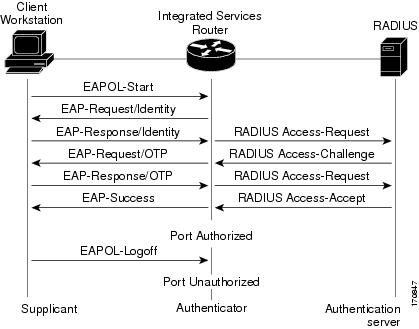
\includegraphics[width=.9\linewidth]{/home/itapuro/gitdocs/di/images/170847.jpg}
\caption{\label{fig:cisco-802.1x}Cisco's view of 802.1x access control with EAP [To be removed from final]}
\end{figure}






\begin{figure}[htb]
\centering
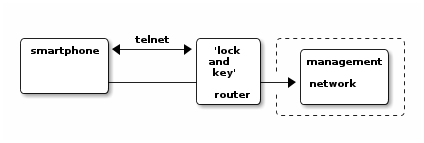
\includegraphics[width=.9\linewidth]{lockandkey.png}
\caption{\label{eap-sim-testbe}Cisco's view of Lock-and-key access}
\end{figure}
\begin{figure}[htb]
\centering
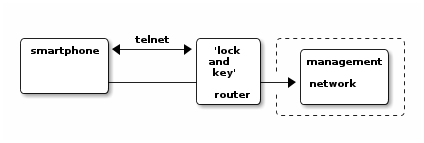
\includegraphics[width=.9\linewidth]{lockandkey.png}
\caption{\label{eap-sim-testbe}Cisco's view of Lock-and-key access}
\end{figure}




Device provider Cisco calls this
 ``Lock-and-Key''\cite[p.117]{lockandkeybook}
access and uses dynamic access list to implement it.
Difference here is that 802.1X protects access to the network in Layer
2 while Lock-and-Key needs to have a functional Layer 3 to conduct
authentication phase.
Figure\ref{fig:cisco-802.1x} reminds us, how 802.1X works.

 Smartphone has only limited access to the network before AA
has completed, while in the Lock-and-key
the other parts of network are already open and successful login to the router opens
access to even more segments through it. In other words, Lock-and-Key
protects IP-access in layer-3 , while 802.1x protects layer-2.
Both methods can have RADIUS as an Authentication server. 
When RADIUS is not available, for example because internet is down,
there almost always exist as a failover a local password method in the configurable 
router.




[This belongs to multiple SSID section]

If Lock-and-key method was used instead of EAP-SIM RADIUS, then
separate management LAN would not be needed. Roles were given at
Authentication server or designated router after mobile has done login to it
via normal access network.



This thesis suggest a mix of these methods: EAP-SIM 802.1x WPA2 for
getting in the management segment \ldots{}



\begin{enumerate}
\item Smartphone connects wireless AP
\item AP, as RADIUS client, connects ROUTER (with Lock-and-key)
\end{enumerate}

Now connection,  from smartphone to configured router is open and 
smartphone may try to login there.

\begin{enumerate}
\item smartphone use telnet (or ssh) to login to the ROUTER.
\item ROUTER(as RADIUS client) checks AA from AP(working as
proxy)
\item AP knows what? It wants to give access, but can it map this request to
earlier facts?
\end{enumerate}
\section{Chosen solution [OR Summary of the chosen solution]}
\label{sec-4-9}

[wrap up of solution]

The chosen solution to benefit from SIM is via EAP-profiles, as EAP
is well known when using WPA2-Enterprise protection in Wi-Fi.

Design is [move from above]\ldots{}
and it is a variation of lock-and-key design.

Above it was mentioned, that the local controller delivers changes to each
device. On this work, it is assumed that the local controller (smart
phone) only \emph{approves} changes,
and delivers them to \emph{one, central CPE}, 
which handles distribution of changes to other CPEs.
Furthermore, the Authenticator is presented as the access point and
RADIUS client (in scenarios I-V), which receives RADIUS messages from
Authentication server, even when there would be a separate local RADIUS server
running as a proxy.
Lastly, a variation of the design is, that not every change needs to go
 through  the local controller and so the process does not always need
interaction from the user.



Critical changes are those, where network topology changes so
that different players would get access outside their earlier domains.
Different players include external service providers, users at home,
visitors, and also home net owner. Examples of the previous cases can first be
seen on the division of homenet to guest and private network and
extensions for homeworkers instead of office.


\chapter{Implemented Solution}
\label{sec-5}


To prove that the proposed model works, empirical tests have been done.
First it is shown how EAP-SIM authentication works. Then a use case for
adding an admin user is reported. Changes are in the end done 
for example with NETCONF from the management network.

\section{EAP-SIM authentication test bed}
\label{sec-5-1}



Used physical devices were two smartphones, an AP and a laptop.
The smartphones were Nokia E70-1 and Nokia E90, both capable of EAP-SIM.
The AP was running OpenWRT firmware.  
Laptop's software were WPA2-Supplicant for Wi-Fi 802.1X access,
hostapd for wired connected RADIUS server and hlr\_auc\_gw for MNO's
HLR-AuC. Laptop's role was therefore physically split-brain: It asked from itself for AA. 
Figure\ref{eap-sim-testbed} shows how EAP-SIM AuthN messages (dashed
and solid arrowed lines) flow when using 
simulated WPA2-Supplicant and HLR-AuC as simulation environment.

\begin{figure}[htb]
\centering
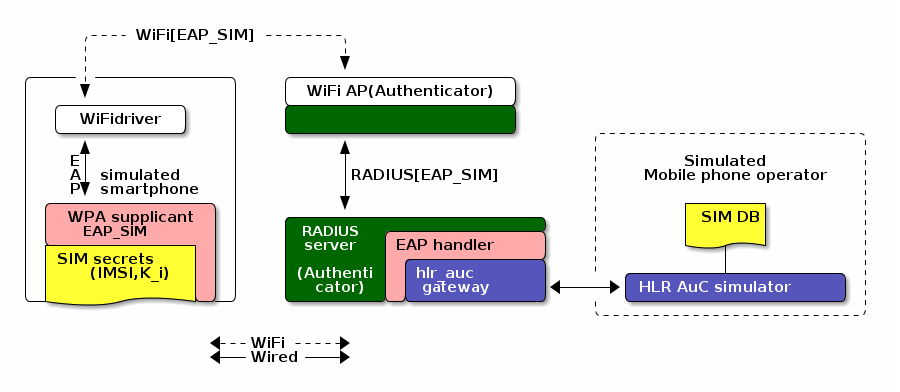
\includegraphics[width=.9\linewidth]{demoinfra.png}
\caption{\label{eap-sim-testbed}EAP-SIM AuthN messaging in simulation testbed}
\end{figure}




Jouni Malinen's software package \emph{HostAP}\cite{hostapd} can be thought
 as a reference
implementation providing all necessary components: WPA2-Supplicant, Wireless
Access point (AP), HLR-gateway (for GSM networks) and EAP-endpoint with
or without RADIUS-server. HSS would replace HLR in 3G/UMTS networks.
The version used in the tests was 2.2, while version
2.4 was published on March 2015.

For a more realistic test, OpenWRT AP is used instead of \emph{hostapd}'s
access point and \emph{hostapd} provides only RADIUS server.
OpenWRT AP works as a RADIUS client connecting to RADIUS server. 
It will not try to open EAP-messages or need
to know about them; it just encapsulates them into RADIUS packet.

The algorithm used in the demo was internal GSM-Milenage,
which handles beside EAP-AKA also EAP-SIM.
Milenage is a reference implementation and as such suitable for operators, who do not 
want to invent their own security algorithms. OPc and Seq numbers,
which are needed in when using EAP-AKA, were not used.

\section{Detailed description of test runs}
\label{sec-5-2}






Test runs were made with diverse clients.
Nokia E70-1 with Symbian 60 Series OS (2006) had a
non-registered SIM card. Despite that it took part in generating
primary EAP traffic.
Examples in appendix \ref{app:nosim}   [TBD]

First tests 
did not go as planned. There was no indication of SIM method
present in captures, the only indication of security was message
``Open System'' in application logs, which means that no pre-shared
key is used.
Nokia E90, with a registered SIM had better results. Traces
are in folder \verb~gitdocs/di/testit/~ files \verb~eap3.pcapng~,
  \verb~e90.sim.auth.pcapng~ and \verb~eap-1.pcapng~  [TBD]

After some modifications, runs got to the authentication phase.
Naturally, challenge-responses did not work because SIM secrets were
not known. Nevertheless, both card succeeded to the point, where MNO's
message would be verified with the SIM card.

Unregistered phone could not use SIM card while 
registered phone verifies and notices, that operator is not right, 
and therefor ends conversation as should be regarding protocol-document [EAP-SIM].

At this point, physical phones were put aside and simulated SIM-card
was used.
After WPA2-Supplicant run on laptop with simulated SIM-card access 
with SIM/USIM protocols, respective EAP-SIM, logging 
from hostapd software claimed that ``Hostapd will send SIM/AKA authentication
queries over a UNIX domain socket to an external \verb~hlr_auc_gw~ program.''
Appendix \ref{app:hlraucgw}   shows that traffic.

Tests were run with a shell program (Appendix \ref{app:fulleap}), which
started the needed programs. It also recorded the used configurations, logs,
and traffic captures for later analysis.

\section{Disconnecting the local controller and offline changes}
\label{sec-5-3}
\label{sec:disconnections}
[Limiting time and forced logout, for how long access provided to
management operations, or use fast-auth on following accesses TBD]

After the phone has been successfully connected to the management network,
changes coming from 
the phone can reach routers.  There should be a way to close the session after
the changes has been applied. Originally it was thought, that the session
would stay open only for a limited time, after which the phone would be forced to
logout or thrown away from the management network and that idea should be
kept in mind when the final implementation is made.





Later it was learned, that terminating a session is not included in the original RADIUS protocol.
The root cause is, that messages originating from the RADIUS server
are not defined in the RADIUS protocol and so AP as RADIUS client cannot
receive RADIUS server initiated disconnection messages. 
As a side note, Diameter protocol provides server initiated messaging.
Additional
extensions such as Disconnect and Change-of-Authorization (CoA)
packets, also known as RADIUS Dynamic Authorization or RADIUS
Disconnection Message(DM), have later been brought in\cite{rfc5176}
to the protocol by diverse vendors, but they may not all be implemented on
every device.
Disconnect-Request is sent to UDP port 3799, so Authenticator should
listen also that in addition to RADIUS UDP port 1812.






[ Following AWAY. left from early phases]

Time limited access can perhaps made with session-timeout parameter
in ACCESS-ACCEPT (or ACCESS-CHALLENGE) packet using type field = ``29''.
This parameter tells the Authenticator how many second maximal the Supplicant
can have service. 

[This cannot be type field 29!]  More specifically, what action
Authenticator should do after termination becomes. It has values of
either 0 (default) or 1 (radius request), which would mean that
Authenticator may send new ACCESS-REQUEST to RADIUS server.

But that would eliminate direct authenticate-only RADIUS cases
  [ \emph{were there}
 \emph{any? I do not remember what I meant}
 \emph{by this. Maybe that we needed only}
 \emph{to have authentication for access} 
 \emph{which in turn enables modifications} ]
Is it then that with value 0, Authenticator does not send
ACCESS-REQUEST to RADIUS server, but client still can automatically send it without 
user's acceptance?
\begin{itemize}
\item forced logout, like in captive portals, where RADIUS is not used.
\item no straightforward solution exists within RADIUS
\item AP is programmable with luci, which is used in configuring routers. It also could run some existing WWW-access
portal [-> reference to \hyperref[text:nointernet]{No Internet connectivity} link is
\end{itemize}








[ Back in track: this can be left here ]

Offline changes include cases where the smartphone is not available
 or when internet connection is down.
If connection to internet is down, full SIM authentication will not
work, because it needs co-operation from internet, namely from MNO.
Simple solution would be sending one-time password to a predefined
phone via an SMS, but what entity would then check that and who would
be authorized to send that message?
Authenticating server, which has no internet connection should 
have way to check that one-time password received via SMS is correct.

Solution for this could be co-existing WWW-based authentication, that
is, a web-page where credentials could be entered.
Software would run in AP. Existing solutions for this are for example
Chillisoft or NoCatAuth. 
Therefore open access to the portal site must be provided without
802.1X port based access control.


Full authentication uses IMSI, which is the identity of the phone's SIM.
Fast re-authentication would use temporal identity TMSI, which 
can change each time the AuthN request had been sent. Mapping
is cached on the  Authenticator and the round-trip and handling at HLR is
so eliminated. 

IMSI is 14 or 15 digit long number and presented as a composition
of digits belonging to MCC(2 digits), MNC(2-3 digits) and MSIN(10 digits).
As for TMSI, it is composed of pseudonym and realm part and can be a
string. So, one can send 
\texttt{my-string-which-can-change@…operator.domain} instead of 
IMSI number (or \texttt{IMSI@...…operator.domain}) as an identity. 


\section{Network traces (EAP, SIM, AUTH traffic analysis)}
\label{sec-5-4}
Wireless capture between WPA2-Supplicant and AP was made on
WPA2-Supplicant's end-point, before it left the wireless card. Capture was
not made in monitoring mode, so not all 802.11 details in
data packets were captured\cite{wireshark-capture}.
Because the focus was not in the radio channel but instead in the EAP messaging, that was not problem.


[Captured wireshark sessions give insight here. Analyze them.
Packet capture of successful SIM-authentication with corresponding
parts of logs at WPA2-Supplicant, RADIUS server and packet captures 
802.1X, RADIUS and HLR. ]

\begin{itemize}
\item flow of messages,  timing,  size, attributes
\end{itemize}

Even when authentication conversation would not complete fully,
Authenticator still receives identification claim from mobile. Yet, as
there is no AuthN, no proof of identity exists in that case.

IMSI is sent first time already on the second EAP message from 
WPA2-Supplicant to AP (see Figure\ref{fig:eap-sim-full}, message 2.)
Same in tests made 150123-155714, source:
testit/demot/ap-s150123-155714/
Capture is from the mobile client, when it has received the first EAP
packet from AP.

\begin{verbatim}
Frame 129: 15:57:17.983047
    Type: 802.1X Authentication (0x888e)
    Version: 802.1X-2004 (2)
    Type: EAP Packet (0)
    Length: 5
    Extensible Authentication Protocol
        Code: Request (1)
        Id: 50
        Length: 5
        Type: Identity (1)
        Identity: 
Frame 130: 15:57:17.983223
    Type: 802.1X Authentication (0x888e)
    Version: 802.1X-2001 (1)
    Type: EAP Packet (0)
    Length: 21
    Extensible Authentication Protocol
        Code: Response (2)
        Id: 50
        Length: 21
        Type: Identity (1)
        Identity: 1232010000000000
#+CAPTION: EAP client's response to identity request
\end{verbatim}
We note here, that AP uses version 802.1X-2004 while WPA2-Supplicant responses with
version 802.1X-2001. Here it does not have any noticeable effect.
The identity field's length is not shown here.
It is not coded as a numerical but a string.
That brings flexibility as the identity can include alphabets too. It also minimizes misunderstandings,
if context gets lost.





EAP client's identity is transformed at Authenticator (Figure\ref{fig:eap-layers}) from 802.1X's 
EAPOL format  into RADIUS format and
sent to RADIUS server:
\begin{verbatim}
Frame3: 15:57:17.988616
Radius Protocol
    Code: Access-Request (1)
    Packet identifier: 0xa2 (162)
    Length: 193
    Authenticator: 055ff370b9e793c1e39d375aade8033c
    Attribute Value Pairs
        AVP: l=18 t=User-Name(1): 1232010000000000
        AVP: l=7 t=NAS-Identifier(32): musta
        AVP: l=27 t=Called-Station-Id(30): 66-66-B3-8A-68-B3:simtest
        AVP: l=6 t=NAS-Port-Type(61): Wireless-802.11(19)
        AVP: l=6 t=NAS-Port(5): 1
        AVP: l=19 t=Calling-Station-Id(31): 5C-51-4F-E7-FA-F4
        AVP: l=24 t=Connect-Info(77): CONNECT 54Mbps 802.11g
        AVP: l=19 t=Acct-Session-Id(44): 5491885C-00000037
        AVP: l=6 t=Framed-MTU(12): 1400
        AVP: l=23 t=EAP-Message(79) Last Segment[1]
            EAP fragment
            Extensible Authentication Protocol
                Code: Response (2)
                Id: 50
                Length: 21
                Type: Identity (1)
                Identity: 1232010000000000
        AVP: l=18 t=Message-Authenticator(80): 04ea7e507d72bdb1acf515ef19ac9527
\end{verbatim}
Interesting part is the EAP fragment, having
Identity=``1232010000000000'', but
also RADIUS message itself, where User-Name field has been set also 
to ``1232010000000000''. 
Identity is filled in WPA2-Supplicant both in identity and credential
section so which one is the correct one, or are they both needed?
Maybe this has something to do with identity
values above, or then AP just has followed conventions on converting
EAP into RADIUS message and put identity field into User-Name Attribute Value Pair (AVP).
The last RADIUS (AVP) is 
Message-Authenticator, which presents limited safety against message 
corruption. Limited, because it uses MD5-hashing which is not safe
against malicious use anymore.

[Here conversation]



[see. /home/itapuro/gitdocs/di/testit/demot/ap-s150123-155714]


\chapter{Analysis, Results and Discussion}
\label{sec-6}



\section{Deployment difficulty}
\label{sec-6-1}

To deploy the system, modifications must be done to AP and client.
Additionally, contract must be made with the MNO service
provider producing AuthN [while AuthZ is already taken care of with
the cloud service contract.]  [TBD, leave cloud out ]
For AP, modifications are minimal. Needed settings are
WPA2 mode to WPA2-enterprise, IP-address of RADIUS server providing 
AA, and corresponding shared secret.
For client, Wi-Fi profile must be added: used management SSID,
protection mode 802.1X (or WPA2-Enterprise), and AuthN method EAP-SIM.
Smartphone modifications can exist together with other
profiles  Different SSID makes that separation possible.

\section{Estimating time to authenticate EAP-SIM}
\label{sec-6-2}
Local tests, with software back ends need less than 20ms for one EAP-RADIUS message
exchange between peers. There will be added time needed to scan Wi-Fi
network for correct access point and SIM card's computing
time.
 [Take reference on network authentication part on earlier
tests. Timeout was 3 seconds for that part.]
[Some Figures for authentication times can give comparison to eduroam
or LANGATONWPA2 network through some RADIUS proxies in between home
organization's RADIUS service.]

\section{Costs for end-user}
\label{sec-6-3}
While no service yet exists from MNOs, we estimate their costs based on
Mobiilivarmenne. Using Mobiilivarmenne 
is currently free for clients, if usage is personal, but costs
for service providers are unknown. 
Regarding hardware, costs can mostly be eliminated, while users
already have smartphones and for infrastructure, existing hardware
such as APs can be used.

Using SIM to local Wi-Fi AA adds value to mobile ecosystem.
To further divide possible costs for EAP-SIM usage
is difficult.
EAP-SIM always needs MNO for first authentication,
because only MNO and SIM-card manufacturer know 
what are SIM's K\_i and the used A3/A8 algorithm
for GSM/3GPP/LTE authentication.

It is difficult to see if any commercial provider would implement
SIM-key sharing so, that secret part were divided to a part that
implements AuthN for own operator and to a part, that is free to use by
some other operator.  Instead, the same functionality can be achieved with
Dual-SIM phones, which allow inserting two SIM cards from different
operators in to the phone. By using menu option in phone, or even a
specific prefix code before call, alternate SIM card can be chosen
without booting the phone.
Dual-SIM thus allows change of ID and IMSI without removing SIM card.

There exists also private GSM networks.
Interesting use case have been Chaos Computer Club's international 
CCC-camps\cite{ccc}, where organizers 
provide private GSM network for attendees of conference
by distributing them separate SIM cards for 2 euros.
Even, when GSM network used 1.8GHz radio channel, of interest here is
only that GSM encryption could be used and SIM-card secrets were known to
the organizing operator.
On the other hand, empty GSM cards for testing can cost as much as 
18 euros a piece (webshop-quote\cite{smartjac-testsim}).


\section{Platform specific issues}
\label{sec-6-4}

For clients, there is no need for public key infrastructure (PKI) 
unless EAP-PEAP is used.
There are smartphones, that do not have EAP-SIM yet available.
For example support for
EAP-SIM (and -AKA) methods starts in Android from version 4.x and in
iOS from version 5.x.\cite{sim-support}.


Generally, what is  needed to bring EAP-SIM support to open source
smartphone is \emph{pcsc-lite} for accessing SIM card, wpa\_supplicant for
wpa client, and possible used connection manager (\emph{connman} or
\emph{wicd}). This is in line, what was done in testing, without pcsc-lite
because a file was used instead of a SIM card.





If OpenWRT platform is used, one problem there is the size of
memory which can be less than 32Mutt's.
WPA2 software included in basic OpenWRT installation is small,
but that does not yet include RADIUS server part or EAP-SIM handling.


Software has other limitations. Freeradius2 is not included yet in OpenWRT.
It would also be based heavily on current Perl environment which
itself may be a space hog. 
Currently, as of 1.7.2014, there is no support for EAP-AKA on
freeradius2 even when there was support on version 1.1.4. \cite{freeradius2}.
EAP-SIM is supported.
Yet, Freeradius can be used as Authentication Center (AuC).
Diameter (freeDiameter) can be compiled in OpenWRT. That is good,
because on 3GPP networks Diameter protocol has more support than RADIUS.
If nothing else works, as a backup old-fashioned WWW-authentication
portal can be used for offline authentication.


\section{Security considerations}
\label{sec-6-5}



There can be multiple ways to attack the described methods of
homenet management delegation. The following subsections divide them into
confidentiality (privacy), integrity, and
authenticity. Accessibility is also discussed.
\subsection{Confidentiality (privacy)}
\label{sec-6-5-1}
The purpose of message confidentiality in authentication phase here is
to hide the identity of smartphone and possible delivered secrets from
eavesdroppers. 

Recall from Section \ref{sec:sim-based-auth}, that IMSI is sent in clear 
during the start phase of 802.1X authentication and that is a privacy 
issue, because TMSI, which hides IMSI cannot be used before a session has been set up. \cite[p.66]{rfc4186}.

This can be compared to regular GSM network identity revealing: IMSI
catching is a concept of listening radio network for phones that are
powered on and register themselves to operator via GSM network.  

The
fault lies there, that GSM specification does not require network to
authenticate itself to the phone in thus GSM allows man in the middle
attack device called IMSI-catcher to fake as being a base station.
When mobile phone tries to attach to a fake base station, it reveals its
IMSI number. Further, because the base station is responsible for chosen
encryption, it can order the phone to not encrypt traffic or to use only
weak encryption thus revealing all data, calls, and
texts. Mitigation for IMSI-catching would be to
disable GSM (2G) usage altogether from phone if that is possible.\cite{imsi-heise}.

After first full authentication, client and Authenticator 
know TMSI and can use it in further communication: Authenticator 
is responsible to convert TMSI to IMSI if it later needs to 
ask for full authentication from the MNO.


If SIM is used as the only EAP without EAP-PEAP, then 
there is no mitigation for revealing the IMSI on the first message
and it leads to privacy issue.

Most(if not all) EAP methods do not provide identity protection
themselves. Protected versions
use separate  inner and outer identities and that can be achieved with
PEAP (Protected  EAP) or TTLS, which chains different EAP-methods together and
protects the inner EAP with an outer EAP. For example 
EAP-MSCHAPv2 (Microsoft's Challenge Handshake Authentication Protocol,
version 2) can be used inside PEAP.
The outer identity tells just the realm, where AuthN can be checked
 and inner identity reveals the real identity.
The inner identity is encapsulated inside the outer identity which
functions as an envelope. [TBD: speak more with protocol terms?]


Used method to authenticate depends on the inability to fake IMSI.
EAP-SIM would provide identity protection, if it were used together
with PEAP which protects the outer identification  and
then EAP-SIM were used in inner authentication.
Currently it is not known for the author that implementations exists for
EAP-SIM  except Tseng's proposition \cite{tseng-usim} for  new EAP type
EAP-USIM, which extends EAP-TLS type.

If it were possible to use anonymous identity on outer EAP
authentication, then EAP-SIM AuthZ must also be done at HLR AuC.
AuthZ cannot else be connected to the corresponding
identity and AuthN itself is not enough because it only defines the users'
authenticity, not their admin roles and so 
AuthN should work for any mobile that has existing contract with
their MNO. 
It still is the responsibility of the Authenticator to 
check AuthZ  and let only admin mobile access the management network.









Based on those facts, EAP-SIM cannot be considered confidential for identity
during first message exchanges, but later the identity can be hidden
using temporal identity (TMSI). Unfortunately, the TMSI is not used in
this thesis for AuthN. 
On the other hand, EAP-SIM protocol, as do most of the other
EAP-variants, provides a secure way to
generate session parameters to WPA2-session and those are not leaked
outside, because they are created individually on both endpoints; 
at smartphone and at AP.
\subsection{Integrity}
\label{sec-6-5-2}
Integrity issues were handled in RADIUS Section \ref{sec:radius}.
Message digestion codes provide integrity for RADIUS protocol.
If PEAP is used, it handles integrity through its usage of TLS
\cite{peap}.

\subsection{Accessibility, DoS and Scalability}
\label{sec-6-5-3}
Is homenet immune against (distributed) denial of service (DoS)
attacks? Besides DoS, does the solution scale up from homenet to
small and middle size companies?
To answer this we can remember that backends (cloud and operator) are
designed for thousands or even millions of concurrent users, so 
they hardly are limiting factors. Instead, local
Authenticator might suffer from inefficiency, which
comes from processing loads\cite{2009-lin-simefficiency}.


Traditionally, RADIUS has used connection\-less UDP protocol for its
light weightiness. UDP misses reliability, but retransmission in UDP is
tolerable, because user is ready to wait several seconds for
authentication to complete. Today, RADIUS can also run over TCP, which
has generally more aggressive retransmission
rate \cite[Section 2.2.1]{rfc5080}. 
On the other hand, adding an
alternative UDP RADIUS server can answer faster than waiting for TCP's reliable delivery.


\subsection{RADIUS weaknesses and strengths in limited use cases}
\label{sec-6-5-4}


RADIUS protocol itself is old and not very secure as of current
standards(2015), because messages are not encrypted and they are
transported on datagrams (UDP). Alternative RADSEC protocol uses TLS, and 
is backwards compatible with RADIUS protocol, so it can be used
as secure RADIUS proxy such as \emph{radproxy}\cite{uninett-radproxy}.

RADIUS uses MD5 hashing and shared secrets. Because of the weaknesses of
MD5 hashing (MD5Attack\cite{rfc5176}), the transport needs additional
protection like tunneling or IPsec. TLS can be used for encryption and
its signatures for integrity checking of packet payload.
RADIUS protocol itself provides some integrity checks with Message
Authenticators as described in Section \ref{sec:radius-macs}.



In scenario III(Figure\ref{fig:scenario-III}),  there was a proxying RADIUS between Authenticator
and MNO.  When MNO notifies Authenticator
that a smartphone has been authenticated, then Authenticator (AP, functioning
as a RADIUS-client) hooks that message and usually just grants
smartphone the access to the network. After giving access rights, other
provisioning parameters can be sent with RADIUS messages, for example
session time-out,
current admin user list, state of OTP list, or VLAN id.


\subsection{Replay, Re-use, Re-auth, and brute-force challenges}
\label{sec-6-5-5}
Earlier in RADIUS analysis, prevention of replied messages was
mentioned. Reusing the same secret in different security context is also
considered bad.  Mixing secrets between usage
domains weakens them.  In GSM networks, IMSI identifies subscriber on
first contact, later TMSI is used for call and SMS.  In EAP-SIM those
values are also used. IMSI naturally is the same, but TMSI should be
different for call and EAP.  Haverinen\cite{hav-doc} explains how
special RAND numbers can be used to differentiate the use of TMSI in 3GPP and LAN
contexts.

Re-authentication and termination can bring unexpected results.
If SSID changing introduced in mitigation Section(\ref{tag:hidessid}) was in use, fast re-authentication
should be forbidden \cite[p.11]{rfc5448}.
Even, when sessions can be terminated, the client side have 
option to login automatically, transparent and without users control.
Automatic re-authentication after disconnection  must be considered
here as harmful as well as automatic login. For example,
Swiss mobile operator Swisscom provided two networks for its customers:
``Mobile'' and ``Mobile Eapsim''. The latter network did not ask customers
for connection and used smartphones' SIMs automatically. Unfortunately,
it also charged users for using Wi-Fi connections without their 
knowledge.\cite{swisscom}





If one can read and write data through SIM card's API,
one could try to get information (SRES, K\_c) by brute-force. 
Fortunately SRES and K\_c are never sent in clear, but inside
a digested MAC.
 Additionally SIM card can be programmed to answer only
limited number of challenge request, for example 65535, which in
normal usage would be enough, but in brute-force challenges 
it would soon be exhausted and not function anymore.


\subsection{Mitigation methods}
\label{sec-6-5-6}
To mitigate risks for radio capturing, two methods are presented: hiding of
wireless network and proximity. They are not perfect but can
limit attack vectors in time and place.


Recall that the management network is needed only then when changes
are challenged. Why then not just enable management radio network
then? Then there were less networks for users to choose from.
Enabling management network could be programmed through OpenWRT router's 
lUCI-interface but preliminary tests showed, that it also 
disconnects existing Wi-Fi connections and may even restart AP,
which certainly would not be wanted. Some other methods need to
be invented to avoid denial-of service.

\label{tag:hidessid}
One could also think of hiding the network by disabling the
advertisement of management network SSID. That is called ``network
cloaking''.  Smartphone would then need to know the exact target SSID name.
The SSID could also be renamed always, in essence
to implement one-time-only network, but then the smartphone would
need to get that secret somewhere, perhaps via an SMS, and then again
that would defeat the purpose of easy access.

Does disabling or hiding the management network bring real security or
is it just security by obscurity?  Security by obscurity means here,
that hiding network would be the only security method.
Disabling or hiding  merely gives one security layer more so it is not
a real security method.

When the usage here is to always renew SSID name then hiding actually
could add security. If the client knows beforehand the name of SSID
(and maybe also AP MAC), then AP does not reveal any information,
before the client has tried to connect to it and that would minimize
the time window for attacks.  Hiding can also have privacy enhancing
effects: Lindqvist's study\cite{hidden-wlan} presents usage of hidden
APs to protect privacy of clients. While Wi-Fi client's normal action is to
probe for SSIDs of lately learned APs, analyzing those probes can reveal client's
earlier locations.



Regarding boundaries of homenet, the Wi-Fi coverage gives 
one natural limit, which is 50 meters indoors or 100 meters outdoors,
when no extenders (i.e. repeaters) are in use.
Proximity so brings a minimal extra layer for preventing attacks
just like network cloaking as the attacker must be physically within those limits.


This can be considered as an added factor in multifactor
authentication or reputation, but it will not be enough, because
attackers will have more sensitive  radios available than normal users
devices have. 
Also, if SIM-profile were used through Bluetooth, there were also
range limits, but even shorter.


\subsection{Decision point for adding role information [ move to design part]}
\label{sec-6-5-7}













Email (2014/Sep) from Karri Huhtanen revealed another
problem (translation by author):
\begin{quote}
``It is possible to add authorization message in-flight in to the
ACCESS-ACCEPT.
Problem is only that, if it is done in flight, you need some way to
combine authentication messages to same identity. SIM auth makes it
possible to use for example temporary identity and then the only thing
what you can mine from the authentication message is the used operator.''
\end{quote}

So proxying RADIUS server cannot know for sure anything but the
originating server (operator) if TMSI is used. The Authenticator does
know the original user, but needs to get AuthZ information. It can get
AuthZ either from the remote operator which would be easier for the
Authenticator or there might be a proxying RADIUS, which inserts that
knowledge into ACCESS-ACCEPT packet. The latter has issues with
temporal identities. 






When proxying RADIUS gets the temporary SIM-identity (TMSI) instead of
a beforehand known IMSI identity, there will be problem
on inserting the admin role information in RADIUS message.
Operator or proxying RADIUS 
does not necessary know about roles without BaaS, so a link
is needed between them to get role information inside RADIUS packet.
It seems, that AuthZ data must be mapped during the first phase of
EAP-SIM AuthN, when IMSI still is available, and in some way
that map must be forwarded to the proxying RADIUS servers.
These issues are fully avoided only in that scenario presented in Chapter
\ref{sec-4}, where there is local Authentication server in homenet.
Partly avoidance can be reached, when only Full Authentication is
used, i.e., authentication is always checked from MNO and no fast
re-authentication is used.

\section{Discussion}
\label{sec-6-6}

[don't jump in with so short flash messages. This looks like conclusion.] 
The environment is modern complex home network management.
Configuration management tools are 
external in the cloud. Trust between homenet and cloud is searched.
Smartphone lies in the intersection of both domains 
and possess properties to simplify binding of that trust.
SIM card of smartphone, used together with Wi-Fi access to homenet 
verifies change controls. For verification, there are few options presented.

Location of AuthN and AuthZ components may also vary.
Always in the beginning, AuthN lies outside homenet, but
later it can use local point. AuthZ may be located more freely.
RADIUS directs user into own virtual LAN segment (VLAN),
and there management of homenet devices is allowed.
That procedure activates the management port as 802.1X standard
specifies.
Thesis thus uses old, yet simple method for problem risen in modern environment homenet.

Disconnection from normal (Wi-Fi) access network happens, before phone can get
into management network. It means, that all stateful network
connections using Wi-Fi will close at that point. Smartphones do not
have multiple wireless connections, but mobile data connections may 
stay up. Even then, the default routing in the smartphone may change.

In the theory chapter it was questioned whether proxying RADIUS server
can read and alter messages on their way or is the messaging secured
by encryption, integrity hashes and digital signatures.
Later it was learned, that message's integrity is protected but not encrypted.

EAP does by definition only AuthN part although successful
authentication often precedes ad hoc AuthZ if nothing is demanded.
EAP-SIM handles this part, but for AuthZ something else is needed
and so some methods has been presented to add right role to 
authenticated identity.

There are many attributes in RADIUS vocabulary, which could be 
used to carry extra information in AuthZ phase. Exactly what 
of them is used remains to implementer's  decision.

Regarding provisioning, it can mean adding users to home with correct
attributes including authentication method and identification.
There pre-existing binding between user and SIM card is carried out
already. 
It also can mean later identifying users and giving them 
dynamically more attributes and access rights.


\chapter{Conclusion}
\label{sec-7}




Homenet's future needs in configuration management have been
described.
 As an example, the change of authority and the delegation of
control to third parties are needs that have been presented.  
A method to approve changes indirectly has been proposed. The approval
follows from successful authentication and authorization with EAP-SIM
method by mobile phone.


Complexity of existing models in interworking was one motivator for
the work. Research work on the subject did reveal some of the reasons 
for the complexity, that are difficult to overcome with simplistic 
methods without in the same time losing security.

As results, a real working EAP-SIM test bed with fake credentials and
fake mobile operator representing EAP-SIM authentication flow has been
shown.  A dual-role model, which binds a smartphone to the homenet and
grants rights to make changes has been proposed.  
An
indirect way to approve changes is achieved by binding the authorized
access to the management network.]

There are some obvious weakness in the proposed solution. Possible usage
must carefully check the safety limits even when RADIUS protocol still
has strengths in security today. The thesis only scratches bootstrapping
problems and issues in bootstrapping the homenet needs to be studied
more thoroughly. One could use tickets in Kerberized way as in GBA.
Software implementation as app is needed to the smartphone.

With the proposed technique, provisioning of users at homenets would
minimize, as users already own an identifiable object, smartphone. As
a positive side effect, two-factor AuthN strengthens existing security.
Developing HS2.0 a few steps further would bring mobile phone internet
off-loading on Wi-Fi networks and that would be the missing link in
interworking between two worlds.

\newpage
%%%%%%%%%%%%%%%
%% BIB
%%%%%%%%%%%%%%%
\bibliographystyle{IEEEtranS}   % already on org header 

\renewcommand{\bibname}{Bibliography}     % Otherwise bilingual babel uses Finnish ``Kirjallisutta''. Strange...
\bibliography{refs}    % already on org header

\addcontentsline{toc}{chapter}{\bibname}  % Include this in TOC

\markboth{\bibname}{\bibname} % Set page header

% not needed \printbibliography                  
% a) heading in English

%%%%%%%%%%%%%
%% APPENDIX
%%%%%%%%%%%%
% if needed, appendix
\appendix
\pagestyle{headings}
%
% a) Not-so-handy way, but at least it works
% 
\def\appA{APPENDIX A. Scripts, confs, and logs} % Define the name and numbering manually
\chapter*{\appA}                       % Create chapter heading
\setcounter{chapter}{1} % Start numbering from zero because command

\markboth{\appA}{\appA}                % Set page header
\addcontentsline{toc}{chapter}{\appA}  % Include this in TOC
% Note that \label does not work with unnumbered chapter

[Appendices are purely optional.  All appendices must be referred to in
the body text, remember this! ]

%\thispagestyle{empty}
\section{shell, logging options}
\label{sec-7-1}
\label{app:fulleap}
\lstset{columns=fullflexible}
# % \lstinputlisting[language=bash]
\lstinputlisting[language=bash]{./testit/apd-tty.clean}



\section{wpa-supplicant creds}
\label{sec-7-2}
[already in text]
If KEYS have been excluded from log files, there as placeholder stays
string ``[REMOVED]''.
\lstinputlisting[language=sh]{testit/wpa-simtest-owrt2.conf.clean}

\section{RADIUS server conf}
\label{sec-7-3}
\lstinputlisting[language=sh]{testit/hostapd-jmdemo.conf.clean}
\section{hlr auc}
\label{sec-7-4}
\label{app:hlraucgw}

\section{No sim}
\label{sec-7-5}
\label{app:nosim}

Here capture + analysis from nosim


\end{otherlanguage} % End on 2nd language part (figures)
\chapter{[MISC to be added on right places]}
\label{sec-8}
\section{facts TBD.}
\label{sec-8-1}
\begin{itemize}
\item ``most EAP authentication protocols lack two features: identity
protection and withstanding man- in-the-middle attacks. ''
\end{itemize}
source :

Yuh-Min Tseng Department of Mathematics, National Changhua University of Education,
Jin-De Campus, Chag-Hua City 500, Taiwan, ROC.

``USIM-based EAP-TLS authentication protocol for
wireless local area networks''
and 

Wireless (In)Security www-page, where 
EAP table shows that PEAP has MiTM.
\url{http://networking.ringofsaturn.com/Security/WirelessInSecurity.php}

\begin{itemize}
\item re-auth for long-lived sessions or if there is cost for disrupting them
\item APs provide different authentication suites for different
\end{itemize}
SSIDs 
\begin{verbatim}
essid="nurkka"
          IE: IEEE 802.11i/WPA2 Version 1
                        Group Cipher : CCMP
                        Pairwise Ciphers (1) : CCMP
                        Authentication Suites (1) : PSK
essid="simtest"
          IE: IEEE 802.11i/WPA2 Version 1
                        Group Cipher : CCMP
                        Pairwise Ciphers (1) : CCMP
                        Authentication Suites (1) : 802.1x
\end{verbatim}
\section{using EAP for other than network access, i.e., for application auth.}
\label{sec-8-2}
\begin{itemize}
\item \url{http://www.rfc-editor.org/rfc/rfc7057.txt}
\begin{itemize}
\item EAP
\end{itemize}
\item application as an EAP peer
\item RFC6677: Channel-Binding Support for Extensible Authentication Protocol (EAP)
\item channel binding must be used
\end{itemize}

\section{eap-psk rfc4764.txt}
\label{sec-8-3}
\begin{itemize}
\item other limitations than identity protection are password support and Perfect Forward Secrecy (PFS).
\item eap-psk
\item only 3 standards track EAP methods per IETF terminology,
\end{itemize}
but all of them are deprecated (md5,OTP,GTC ja?)
\begin{itemize}
\item some EAP- o  Essentially require additional infrastructure, e.g., EAP-SIM \footnote{DEFINITION NOT FOUND.},
EAP-AKA \footnote{DEFINITION NOT FOUND.}, or OTP/token card methods like \footnote{DEFINITION NOT FOUND.}.
\end{itemize}


\section{eap-sim acts similar than any other EAP challenge method (or not?)}
\label{sec-8-4}
\begin{itemize}
\item compare eap-sim with other method and point out differences.
\item privacy already shown
\item user defined passwd?
\item how many messages needed? In eap-sim 6+1 (success/failure)
\item to do comparison, I have to study how EAP in general works
\item Authenticator for example can use either local method or
pass-through the authentication to external backend, still keeping
EAP-message in tact(sp?) as of  rfc4137
\item WPA2 package's hostapd from JM does not perhaps provide EAP-PEAPv0 SIM but
\end{itemize}
wpa-supplicant supports.
\begin{itemize}
\item VLAN itself has an attack vector and some methods exists, but also
mitigation for them.
\item rad Authenticator, TLS, RADSEC etc, needs both client\&server in
x509 certificate
\end{itemize}
% Emacs 24.4.1 (Org mode 8.2.10)
\end{document}